\documentclass[10pt,a4paper]{article}
\usepackage[paper=a4paper, hmargin=1.5cm, bottom=1.5cm, top=3.5cm]{geometry}

\usepackage[utf8]{inputenc}
\usepackage[spanish]{babel}

\usepackage{mathtools}
\usepackage{amsmath}
\usepackage{amsfonts}
\usepackage{amssymb}

\usepackage{xcolor}
\usepackage{listingsutf8}
\usepackage{booktabs}
\usepackage{hyperref}

\usepackage{algpseudocode}
\usepackage{ifthen}
\usepackage{enumitem}

\usepackage[pdftex]{graphicx}
\usepackage{tikz}

\usepackage{epstopdf}
\usepackage[framemethod=tikz]{mdframed}

% set the default code style
\lstset{
    frame=tb, % draw a frame at the top and bottom of the code block
    tabsize=4, % tab space width
    showstringspaces=false, % don't mark spaces in strings
    numbers=left, % display line numbers on the left
    commentstyle=\color{green}, % comment color
    keywordstyle=\color{blue}, % keyword color
    stringstyle=\color{red} % string color
}

\author{}
\title{Organización del Computador II \\ TP2}
\begin{document}

%% cover page

\maketitle

\bigskip

\begin{table}[h]
\centering
\begin{tabular}{|l l l|}
\hline
Integrante       & \multicolumn{1}{c}{LU}     & Correo electrónico        \\ \hline
Federico Beuter & 827/13                      & federicobeuter@gmail.com \\
Juan Rinaudo & 864/13                      & jangamesdev@gmail.com \\ 
Mauro Cherubini & 835/13                      & cheru.mf@gmail.com \\ \hline
\end{tabular}
\end{table}

\vfill

\begin{center}
\textbf{Reservado para la cátedra}
\end{center}
\begin{table}[h]
\centering
\begin{tabular}{|l|l|l|}
\hline
Instancia       & Docente & Nota \\ \hline
Primera entrega &         &      \\ \hline
Segunda entrega &         &      \\ \hline
\end{tabular}
\end{table}

\pagebreak

\tableofcontents

% end cover page

\pagebreak

\section{Introducción}

El objectivo del trabajo practico es utilizar el set de instrucciones SIMD para el procesamiento de imagenes.
Para esto se nos pidio implementar 2 versiones en ASM (x86_64) de 3 filtros diferentes (Blur, Merge, HSL), ademas se nos brindo una version en C para usar como guia.

Es importante destacar que las imagenes que vamos a procesar son multiplo de 4 pixeles y con un tamaño minimo de 16 pixeles, esto nos permite en nuestras implementaciones cargar de a 4 pixeles en los registros XMM sin tener que preocuparnos por los casos borde.
Ademas el procesamiento de las imagenes se hace unicamente usando instrucciones SSE y durante el procesamiento de los mismos tratamos de mantenernos adentro de los margenes de error brindados por los test de la catedra.

Una vez implementado los 3 filtos y sus diferentes versiones se iniciara con la etapa de experimentacion, donde buscamos responder las preguntas brindadas por la catedra y formar un mayor entendimiento de los algoritmos implementados para sacar nuestras propias conclusiones.

\section{Filtro 1: Blur}

\subsection{Cambios}
Para el recuperatorio decidimos hacer cambios en el codigo.

La lista de cambios esta a continuacion, con la aclaracacion de por que se hicieron los mismos:
\noindent
\begin{itemize}
\item Se remplazaron las operaciones que realizaban las copias por operaciones de SIMD para aumentar la velocidad a la que se copian los pixeles, tambien se modifico el codigo el cual antes copiaba las dos filas de pixeles superiores para que solo copie una (Swapeando los punteros de R13 con R12 y luego solo copiando en R13 los datos de la fila de pixeles del medio).
\end{itemize}

\subsection{Explicacion}

El filtro $blur$ consiste en para cada pixel (exceptuando los ubicados en el borde), tomar sus 8 vecinos y hacer un promedio de cada uno de sus componentes \texttt{R}, \texttt{G} y \texttt{B} entre los 9 pixeles, este nuevo valor reemplaza los que teniamos en el pixel actual. El promedio debe ser calculado respecto a los datos originales, es decir, que si al procesar un pixel y alguno de los vecinos ya fue procesado, debemos utilizar los datos del mismo antes de la modificacion. Nuestro algoritmo se basara en el implementado por la catedra en $C$ pero aprovechando de las operaciones vectoriales de SIMD para mejorar su performance tratando de trabajar con la mayor cantidad de datos al mismo tiempo.

\subsection{Implementacion 1}
La primera implementacion nos pide trabajar de a 1 pixel por iteracion.

Los pixeles estan compuestos por 4 bytes: \texttt{A R G B}, esto nos permite cargar 4 pixeles en un registro \texttt{XMM}, como nosotros necesitamos 9 pixeles, ubicados de a 3 en 3 filas diferentes vamos a precisar 3 registros \texttt{XMM} para cargarlos (Para esto usamos los registros \texttt{XMM0}, \texttt{XMM2} y \texttt{XMM4}). Ademas se utilizaron los siguientes 6 registro de proposito general: \\

\noindent
\begin{itemize}
\item \texttt{RDI} que lo usamos para iterar sobre el eje \texttt{X}
\item \texttt{R9} que lo usamos para iterar sobre \texttt{Y}
\item \texttt{R12} que es un puntero a la copia de la fila superior
\item \texttt{R13} que es un puntero a la copia de la fila actual
\item \texttt{R8} es un puntero a la fila inferior
\item \texttt{R10} es un puntero a la fila actual de la imagen (fila que estoy modificando)
\end{itemize}

Esto se puede visualizar en el siguiente grafico:

\begin{figure}[h!]
	\centering
	\includegraphics[scale=0.5]{images/BlurASM1_0}
\end{figure}

Donde \texttt{P} es el pixel a procesar.

Antes de comenzar el ciclo incicializamos \texttt{RDI} en 0, \texttt{R9} en 2, movimos \texttt{R8} a \texttt{R10}, aumentamos \texttt{R8} en una fila y posicionamos el puntero a la imagen en memoria en la segunda fila de pixeles.

Al principio de cada ciclo copiamos en los registros los 3 grupos de pixeles y quedan de la siguiente manera:\\

\noindent
\texttt{XMM0 $\gets$ [R12 + RDI] = - $\vert$ p2 $\vert$ p1 $\vert$ p0}\\
\texttt{XMM1 $\gets$ [R13 + RDI] = - $\vert$ p5 $\vert$ p4 $\vert$ p3}\\
\texttt{XMM2 $\gets$ $\ $[R8  + RDI] = - $\vert$ p8 $\vert$ p7 $\vert$ p6}\\

Despues desempaquetamos los pixeles de $byte$ a $word$ para poder sumar los 9 pixeles sin saturacion, hicimos una copia de cada uno para poder desempaquetar la parte inferior en un registro y la superior en otro (\texttt{XMM1 = XMM0}, \texttt{XMM3 = XMM2}, \texttt{XMM5 = XMM4}) y ademas llenamos un registro (\texttt{XMM12}) con ceros para expandir cada una de las componentes sin alterar el numero original.
Una vez desempaquetados nos quedan los registros con los siguientes valores:\\

\noindent
\texttt{XMM0 $\gets$ p1 $\vert$ p0} \\
\texttt{XMM1 $\gets$ - $\ \vert$ p2} \\
\texttt{XMM2 $\gets$ p4 $\vert$ p3} \\
\texttt{XMM3 $\gets$ - $\ \vert$ p5} \\ 
\texttt{XMM4 $\gets$ p7 $\vert$ p6} \\
\texttt{XMM5 $\gets$ - $\ \vert$ p8} \\
\\
Luego sumamos los registros e hicimos la division. \\

Sumando \texttt{XMM0}, \texttt{XMM2} y \texttt{XMM3} en \texttt{XMM15}: \\
	\texttt{XMM15 $\gets$ p1 + p4 + p7 $\vert$ p0 + p3 + p6}	\\

Sumando \texttt{XMM1}, \texttt{XMM3} y \texttt{XMM4} en \texttt{XMM14}	\\
	\texttt{XMM14 $\gets$ - $\vert$ p2 + p5 + p8} \\

Luego hicimos una copia de \texttt{XMM15} en \texttt{XMM13} y la shifteamos 8 bytes a la derecha \\
	\texttt{XMM13 $\gets$ - $\vert$ p1 + p4 + p7} \\

Por ultimo sumamos \texttt{XMM15}, \texttt{XMM14} y \texttt{XMM13} en \texttt{XMM15} \\
	\texttt{XMM15 $\gets$ - $\vert$ p0 + p1 + p2 + p3 + p4 + p5 + p6 + p7 + p8} \\

Para hacer la division optamos por multiplicar por $(2^{16} / 9) + 1$ y luego shiftear 16 bits a la derecha cada componente. Para eso tengo el valor por el cual voy a multiplicar en memoria precalculado, al principio del programa decidimos guardarlo en \texttt{XMM11}.
Luego, hicimos una copia de \texttt{XMM15} en \texttt{XMM14} y multiplicamos por \texttt{XMM12} guardando la parte superior de la mutiplicacion en \texttt{XMM15} y la inferior en \texttt{XMM14}. Luego empaquetamos los dos valores juntos como doubleword y los guardamos en \texttt{XMM14} y shifteamos 16 bits a la derecha.
Por ultimo empaquetamos los valores obtenidos a words y luego a bytes, posteriorment los guardamos en la posicion de memoria del pixel actual.

Aumentamos en 4 el iterador en \texttt{X} y comparamos con el tamaño en bytes de una linea de pixeles, si es menor iteramos nuevamente. En caso de que fuese mayor o igual, copiamos cambiamos los punteros de \texttt{R12} y \texttt{R13} y luego copiamos en R13 los pixeles de la siguiente fila (las cuales seran necesarias para poder operar la siguiente fila).

Para terminar copiamos \texttt{R8} en \texttt{R10}, movemos \texttt{R8} una fila de pixeles, reseteamos el iterador X \texttt{RDI}, incrementamos el iterador en Y \texttt{R9} y si el iterador de Y es menos a la altura de la imagen iteramos nuevamente.

\subsection{Implementacion 2}
Para la segunda implementacion se nos pidio trabajar de a 4 pixeles por iteracion.

Para eso calculamos primero los pixeles \texttt{P0} y \texttt{P1}, y despues el \texttt{P2} y \texttt{P3} tratando de minimizar la cantidad de accesos a memoria. \\

\begin{figure}[h!]
	\centering
	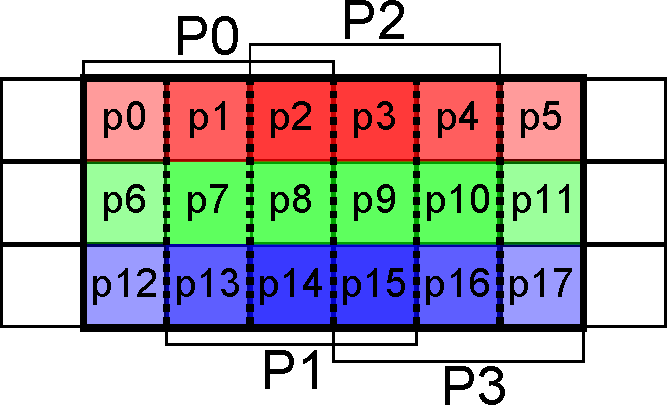
\includegraphics[scale=0.5]{images/BlurASM2_1}
\end{figure}

Para hacer los calculos tomamos 6 set de 4 pixeles que nos permiten sumar en un solo registro 2 pixeles al mismo tiempo usando solo sumas, cada set ira adentro de un registro \texttt{XMM}. Ademas necesitamos 6 registros \texttt{XMM} mas para poder desempaquetar los bytes a words, y asi no tener saturacion. \\

\newpage
Al igual que la primer implementacion, necesitaremos los mismos 6 registros de proposito general. \\

\begin{figure}[h!]
	\centering
	\includegraphics[scale=0.5]{images/BlurASM2_0}
\end{figure}

Antes de comenzar el ciclo incicializamos \texttt{RDI} en 0, \texttt{R9} en 2, movimos \texttt{R8} a \texttt{R10}, aumentamos \texttt{R8} en una fila y posicionamos el puntero a la imagen en memoria en la segunda fila de pixeles.

Luego cargamos los 6 pixeles a sus respectivos registros:\\

\noindent
\texttt{XMM0 $\ \gets$ p3 $\ \vert$ p2 $\ \vert$ p1 $\ \vert$ p0} \\
\texttt{XMM2 $\ \gets$ p4 $\ \vert$ p3 $\ \vert$ p2 $\ \vert$ p1} \\
\texttt{XMM4 $\ \gets$ p9 $\ \vert$ p8 $\ \vert$ p7 $\ \vert$ p6} \\
\texttt{XMM6 $\ \gets$ p10 $\vert$ p9 $\ \vert$ p8 $\ \vert$ p7} \\
\texttt{XMM8 $\ \gets$ p15 $\vert$ p14 $\vert$ p13 $\vert$ p12} \\
\texttt{XMM10 $\gets$ p16 $\vert$ p15 $\vert$ p14 $\vert$ p13} \\

De la misma forma que en la primer implementacion desempaquetamos los registros haciendo una copia y desempaquetando la parte superior en el registro original y la inferior en la copia. Para desenpaquetar usamos un registro con ceros (\texttt{XMM15}) \\

\noindent
\texttt{XMM0 $\ \gets$ p1 $\ \vert$ p0} \\
\texttt{XMM1 $\ \gets$ p3 $\ \vert$ p2} \\
\texttt{XMM2 $\ \gets$ p2 $\ \vert$ p1} \\
\texttt{XMM3 $\ \gets$ p4 $\ \vert$ p3} \\ 
\texttt{XMM4 $\ \gets$ p7 $\ \vert$ p6} \\
\texttt{XMM5 $\ \gets$ p9 $\ \vert$ p8} \\
\texttt{XMM6 $\ \gets$ p8 $\ \vert$ p7} \\
\texttt{XMM7 $\ \gets$ p10 $\ \vert$ p9} \\
\texttt{XMM8 $\ \gets$ p13 $\ \vert$ p12} \\
\texttt{XMM9 $\ \gets$ p15 $\ \vert$ p14} \\ 
\texttt{XMM10 $\gets$ p14 $\ \vert$ p13} \\
\texttt{XMM11 $\gets$ p16 $\ \vert$ p15} \\

Con todos los registros cargados, procedimos a sumar cada uno de ellos con XMM15, el resutlado final fue el siguiente:\\

\noindent
\texttt{XMM15 $\gets$ p1 + p2 + p3 + p7 + p8 + p9 + p13 + p14 + p15 $\vert$ p0 + p1 + p2 + p6 + p7 + p8 + p12 + p13 + p14}\\

Como podemos apreciar, el mismo responde al grafico presentado anteriormente, particularmente a los pixeles \texttt{P0} y \texttt{P1}. Luego hicimos la division de cada pixel de la misma manera que en la primer implementacion, antes de dividir preservamos una copia de \texttt{XMM15} en \texttt{XMM9}, dividimos por 9, shifteamos 8 bytes y dividimos nuevamente. Finalmente movimos los pixeles procesados a \texttt{P0} y \texttt{P1} a la memoria en la posicion correcta. Despues hubo que procesar los pixeles \texttt{P2} y \texttt{P3}, para hacer esto movimos 3 grupos mas de pixeles de la memoria hacia los registros. En esta etapa tenemos:

\noindent
\texttt{XMM0 $\gets$ p5 $\ \vert$ p4 $\ \vert$ p3 $\ \vert$ p2}\\
\texttt{XMM4 $\gets$ p11 $\vert$ p10 $\vert$ p9 $\ \vert$ p8}\\
\texttt{XMM8 $\gets$ p17 $\vert$ p16 $\vert$ p15 $\vert$ p14}\\

Luego hicimos copias en \texttt{XMM1}, \texttt{XMM5} y \texttt{XMM9} y desempaquetamos de byte a word:\\

\noindent
\texttt{XMM0 $\gets$ p3 $\ \vert$ p2}\\
\texttt{XMM1 $\gets$ p5 $\ \vert$ p4}\\
\texttt{XMM4 $\gets$ p9 $\ \vert$ p8}\\
\texttt{XMM5 $\gets$ p11 $\vert$ p10}\\
\texttt{XMM8 $\gets$ p15 $\vert$ p14}\\
\texttt{XMM9 $\gets$ p17 $\vert$ p16}\\

Nuevamente sumamos los registros de la misma forma que antes, es decir, uno a uno con \texttt{XMM15}, el resultado final es:\\

\noindent
\texttt{XMM15 $\gets$ p3 + p4 + p5 + p9 + p10 + p11 + p15 + p16 + p17 $\vert$ p2 + p3 + p4 + p8 + p9 + p10 + p14 + p15 + p16}

Como podemos apreciar, en este caso las cuentas tambien responden a lo presentado en los graficos, en este caso a los pixeles \texttt{P2} y \texttt{P3}. De la misma forma que antes hacemos las divisiones apropiadas, y guardamos los pixeles procesdos en memoria.

Una vez terminado el procesamiento de pixeles, comparamo el iterador con la cantidad de pixeles en una fila y repetimos hasta llegar hasta los ultimos 16 bytes de la fila, estos ultimos 16 bytes los cargamos en solo 3 registros \texttt{XMM} y los procesamos al igual que la primera parte del ciclo para asegurarme de no pasarnos. Al final del ciclo hacemos las copias pertinentes, incrementamos el iterador de filas y revisamos si llegamos al final. \\

\subsection{Resultados}
Para la experimentacion vamos a correr las 3 implementaciones (La version de C compilada con optimizaciones de nivel 3) para poder comparar la performance, vamos a usar la imagen de $lena$ brindada por la catedra (Resolucion 160x160). Se ejecutara cada implementacion del algoritmo 100 veces y luego se calculara el tiempo minimo, maximo y promedio. A continuacion graficamos los tiempos en un grafico de barras que esta a continuacion:

\begin{figure}[h!]
	\centering
	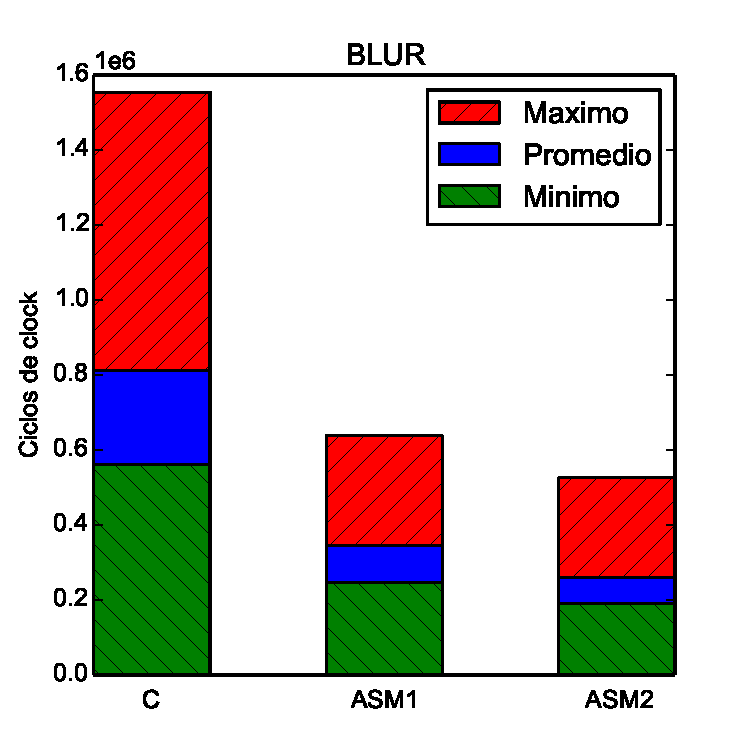
\includegraphics[scale=0.45]{images/blur_comparation}
\end{figure}

Con esto podemos ver que la implementacion ASM2 es un poco mas rapida que las otras implementaciones.

Revisando el codigo podemos ver que el tamaño de la imagen solo deberia modificar cantidad de pixeles a procesar aumentando el tiempo de ejecucion solo por que se necesita hacer mas iteraciones, tambien podemos ver que el algoritmo es independiente del color de los pixeles a procesar.

Para la reentrega se hicieron algunos cambios en el codigo que se supone que deberian mejorar la performance (Ver lista de cambios), decidimos correr el test explicado anteriormente el codigo nuevo y el codigo viejo para comfirmar que los cambios propuestos cumplan con su objetivo. En el siguiente grafico graficaron los tiempos maximos, minimo y promedio de ejecucion de la implementaciones de ASM.

\begin{figure}[h!]
	\centering
	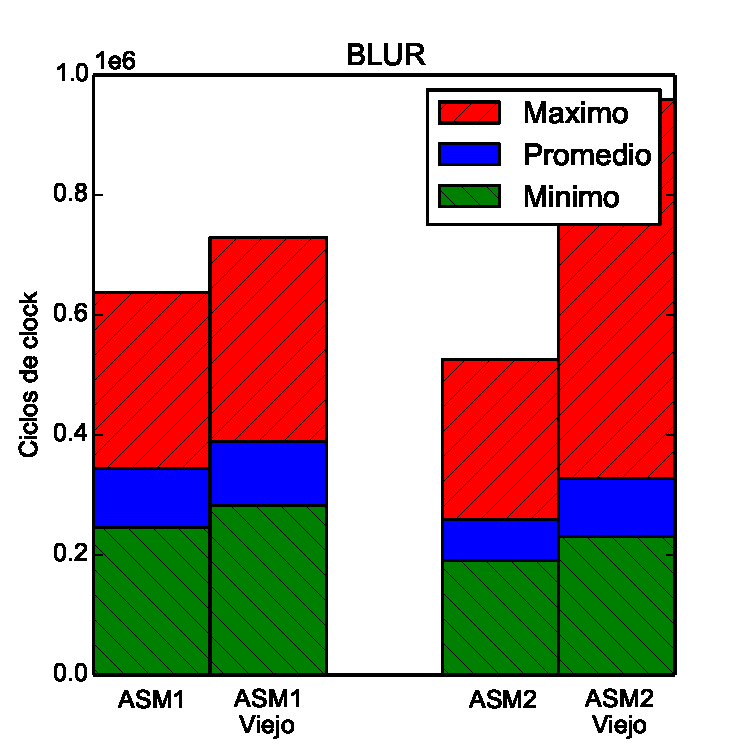
\includegraphics[scale=0.45]{images/blur_comparationOLD}
\end{figure}



\newpage

% Para la experimentacion vamos a correr las 3 implementaciones (La version de C compilada con optimizaciones de nivel 3) con la imagen de $lena$ brindada por la catedra (multiplos de 16x16, hasta 320x320). Cada tamaño se ejecuta 100 veces, despues se saca un promedio y se lo grafica junto con el maximo y el minimo. La metodologia adoptada para evaluar la eficacia de las implementaciones es tomar la cantidad de ciclos que tarda en correr cada una de las implementaciones, esto lo hacemos mediante la libreria \texttt{rdtsc.h}, las pruebas van a ser ejecutadas en un \texttt{Intel Core i7 4700MQ}. Estas condiciones de prueba se mantendran durante el resto del informe y para todos los filtros.

% \begin{figure}[h!]
% 	\centering
% 	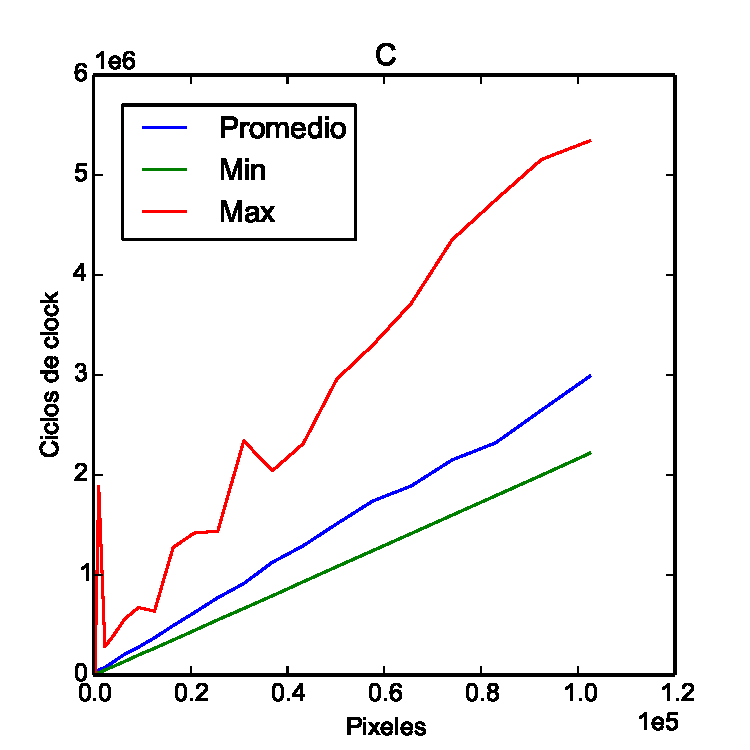
\includegraphics[scale=0.45]{images/c_blur}
% 	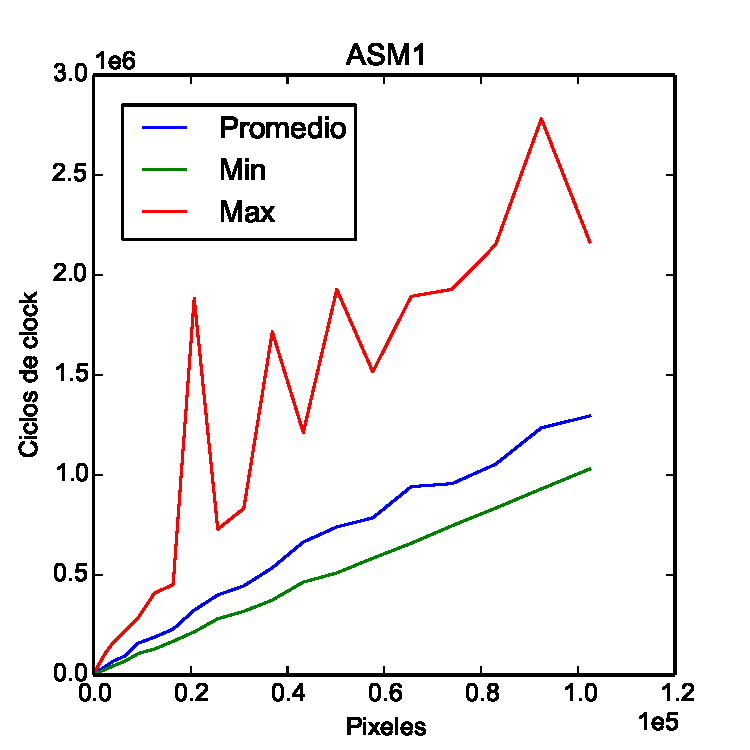
\includegraphics[scale=0.45]{images/asm1_blur}
% 	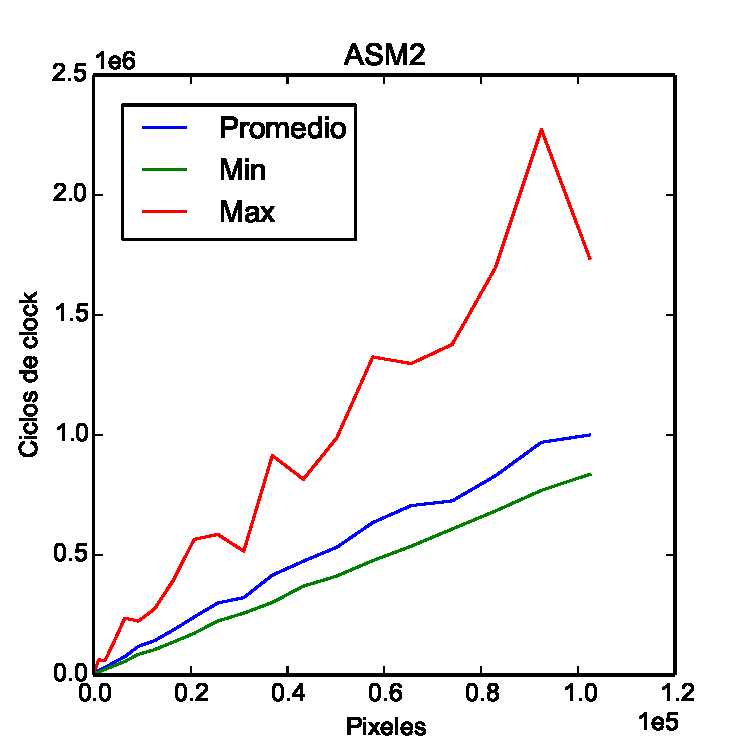
\includegraphics[scale=0.45]{images/asm2_blur}
% \end{figure}

% Ahora graficamos los 3 valores promedios de $blur$ para ver cual de ellos es el mas rapido en general. Para ver mejor la diferencia entre ASM1 y ASM2 los graficamos aparte.

% \begin{figure}[h!]
% 	\centering
% 	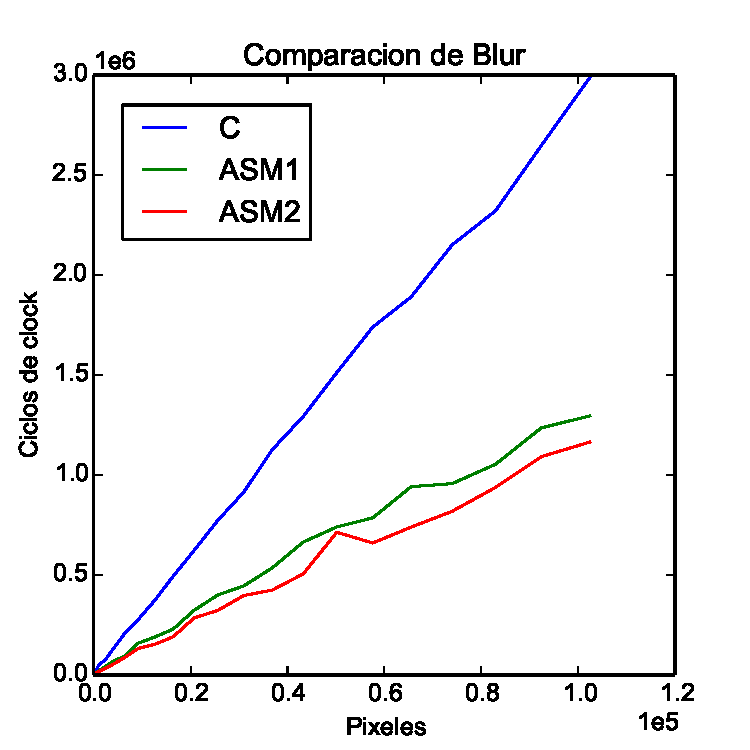
\includegraphics[scale=0.5]{images/c_asm1_asm2_blur_comp}
% 	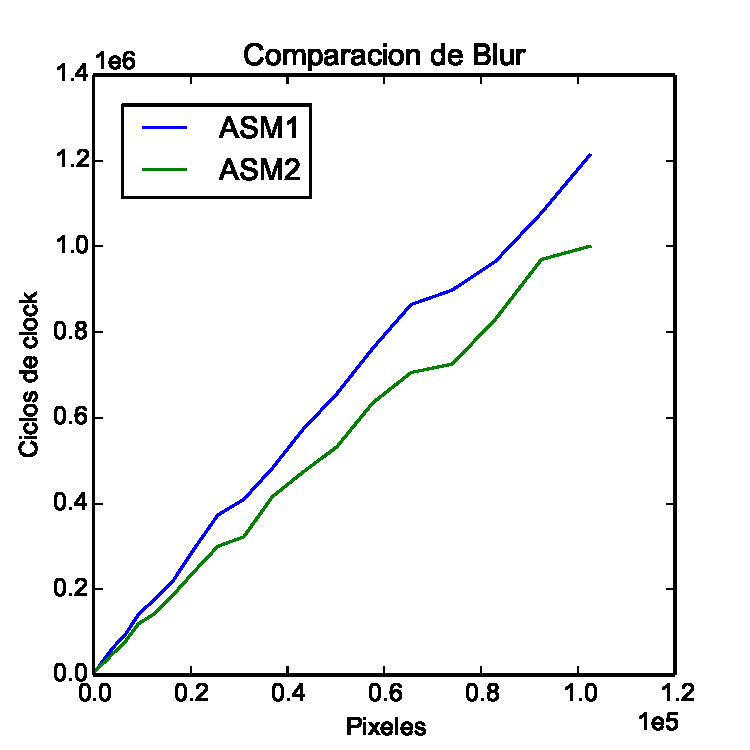
\includegraphics[scale=0.5]{images/asm1_asm2_blur_comp}
% \end{figure}

% Este grafico nos muestra que el codigo de ASM2 pareceria ser el mas rapido. Antes de confirmar esto queremos ver que no haya ningun tipo de factor en la imagen que influya en el tiempo de ejecucion que no sea el tamaño. \\

% Tanto en el codigo de C como en el ASM1 y ASM2 no poseen ninguna operacion que dependa de los pixeles a procesar, para probar que esto es realmente asi en la practica decidimos correr los test al igual que al principio pero esta vez usando la imagen de $lena$, $colores$ y 3 imagenes mas completamente rojas, azules y verdes.\\

% \begin{figure}[h!]
% 	\centering
% 	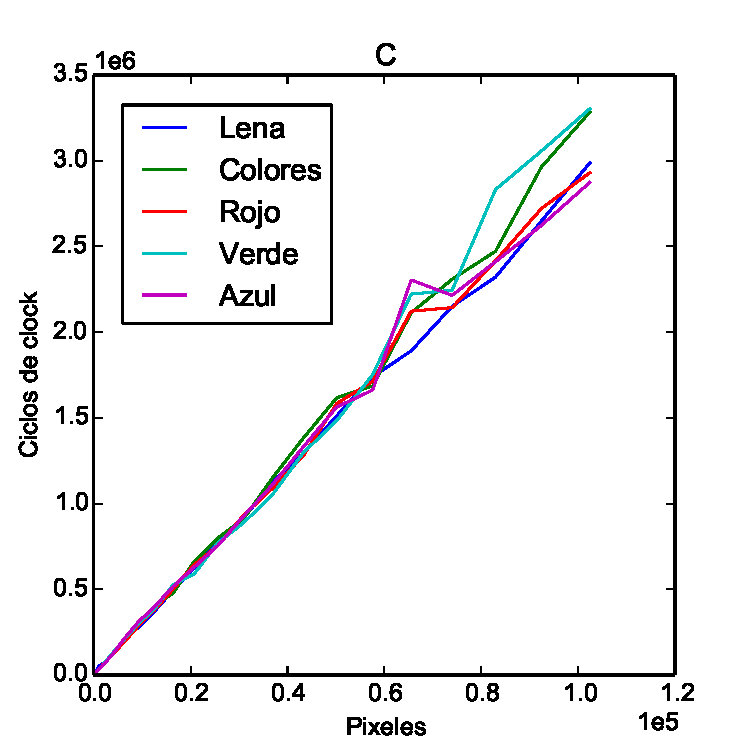
\includegraphics[scale=0.45]{images/c_blur_lena_colors}
% 	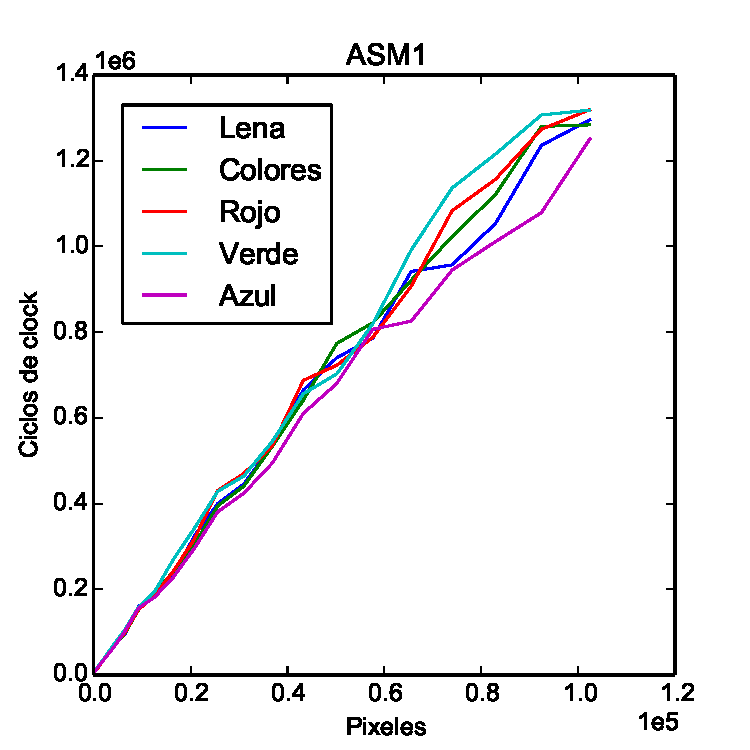
\includegraphics[scale=0.45]{images/asm1_blur_lena_colors}
% 	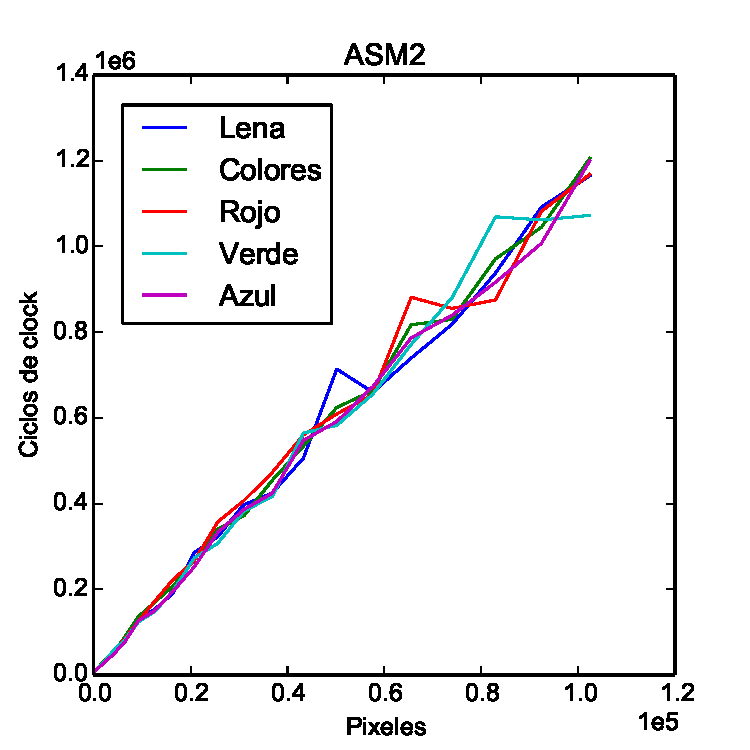
\includegraphics[scale=0.45]{images/asm2_blur_lena_colors}
% \end{figure}

\subsection{Conclusion}
Podemos concluir que en el caso de la utilizacion de instrucciones SIMD para la aplicacion del algoritmo de blur se puede ver que operar de a varios pixeles mejora un poco con respecto a operar de a un pixel pero al mismo tiempo tambien complica considerablemente el codigo que se debio implementar en nuestro caso.

Igual la simple implementacion de instrucciones SIMD comparandola con el codigo C compilado se puede notar una diferencia conciderable en cuanto a la cantidad de ciclos de reloj usados por el mismo.

% Luego de la experimentacion podemos concluir que ASM2 es el mas rapido en general. \\

% La imagen a procesar no afecta en nada el tiempo de ejecucion y el tamaño lo afecta solo por que se deben procesar mas pixeles. \\
\newpage

\section{Filtro 2: Merge}

\subsection{Explicacion}
El filtro $merge$ consiste en tomar 2 imagenes del mismo tamaño y un parametro (llamdo \texttt{value} en el enunciado) de tipo $float$ entre 0 y 1, multiplicar las componetes de la primer imagen por \texttt{value} y los de la segunda por \texttt{1 - value} y sumar los pixeles de ambas para crear una nueva imagen. \\

\subsection{Implementacion 1}
Para la primer implementacion se nos pidio trabajar con valores de tipo $float$, procesando la mayor cantidad de pixeles posibles por iteracion. \\

Ya que la cantidad de pixeles por imagen siempre va a ser un multiplo de 4 segun el enunciado, decidimos tomar de a 4 pixeles de la memoria para trabajar con los mismos, esto nos permitio simplificar el ciclo y operar sin tener que preocuparnos por excedernos del area de memoria alocada a la imagen.\\

Para procesar los pixeles del merge utilizamos 2 registros \texttt{XMM} para guardar los 4 pixeles como bytes que obtenemos de la memoria, y 2 registros mas para guardar copias de los mismos. Ademas como utilizamos una funcion auxiliar tambien precisamos de 4 registros \texttt{XMM} mas para poder guardar los resultados de la funcion. Por ultimo, tenemos \texttt{value} y \texttt{1 - value} guardados en los registros \texttt{XMM15} y \texttt{XMM14} respectivamente. Ademas de estos registros, se emplearon tambien los siguientes de proposito general:\\

\noindent
\begin{itemize}
	\item \texttt{RDX} puntero a la primera imagen
	\item \texttt{RCD} puntero a la segunda imagen
	\item \texttt{R9} iterador en \texttt{Y}
	\item \texttt{R8} iterador en \texttt{X}
\end{itemize}

Esta distribucion de registros reponde al siguiente grafico:

\begin{figure}[h!]
	\centering
	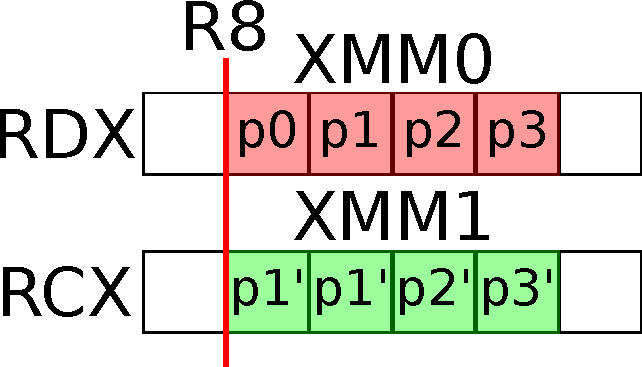
\includegraphics[scale=0.5]{images/MergeASM1_0}
\end{figure}

Antes de empezar a recorrer la imagen, para asignar los valores correctos de \texttt{XMM14} y \texttt{XMM15} utilizamos el dato \texttt{value} original almacenado en \texttt{XMM0}. Este valor fue copiado mediante un operacion de shuffle hacia \texttt{XMM15}, esta operacion copiaba \texttt{value} a todas las componentes de \texttt{XMM15}. Para poder calcular \texttt{XMM14} alcanzo con mover al mismo una constante almacenada en memoria que tuviese \texttt{1.0} en los 4 $float$ y posteriormente restarle el contenido de \texttt{XMM15}. Finalmente tenemos en \texttt{XMM14} y \texttt{XMM15}:\\

\noindent
\texttt{XMM14 $\gets$ 1 - value $\vert$ 1 - value $\vert$ 1 - value $\vert$ 1 - value}\\
\texttt{XMM15 $\gets\ \ $ value $\ \ \vert\ \ $ value $\ \ \vert\ \ $ value $\ \ \vert\ \ $ value}\\

Para poder movernos por la imagen empleamos dos ciclos anidados, el primero de ellos nos permite, junto con \texttt{R9}, iterar sobre el eje \texttt{Y}, mientras que el ciclo interno nos permite movernos con facilidad sobre el eje \texttt{X} mediante \texttt{R8}. Antes de comenzar a iterar en el ciclo principal, incializamos ambos iteradores en 0, y si llegamos al final del ciclo interno (es decir, iteramos sobre todo el eje \texttt{X} para la fila actual) colocamos el iterador de \texttt{X} en 0. Al comienzo de cada ciclo de \texttt{X}, movemos hacia los registros \texttt{XMM0} y \texttt{XMM1} los datos de los pixeles a procesar de la primer y segunda imagen respectivamente, ademas copiamos cada una en \texttt{XMM2} y \texttt{XMM3}, luego de esto procedimos a llamar a la funcion auxiliar \texttt{addPixels} 4 veces. Al finalizar los llamados, tenemos en \texttt{XMM4} los 4 pixeles procesados, lo unico restante fue volcarlos en memoria. Una vez que los pixeles se encuentran en memoria, tenemos que aumentar el iterador de \texttt{X} en 16 bytes, y en caso de haber llegado al final de la fila, colocar el mismo en 0 e incrementar el de \texttt{Y}. Si ya llegue al final de la imagen, termino el ciclo principal de la implementacion y procedo a retornar de la funcion.

La funcion \texttt{addPixels} es una funcion auxiliar la cual hace la aritmetica necesaria para poder mergear las imagenes, esta funcion toma los valores de \texttt{XMM2} y \texttt{XMM3} y los copia hacia \texttt{XMM0} y \texttt{XMM1} respectivamente, luego procede a desempaquetarlos a doubleword utilizando el registro \texttt{XMM10} el cual contiene 0 en todas sus componentes. Una vez desempaquetados los valores, se procede a convertirlos a tipo $float$ para poder realizar el producto con \texttt{XMM14} (\texttt{1-value}) y \texttt{XMM15} (\texttt{value}). Entonces tenemos:

\noindent
\texttt{XMM0 $\gets$ a * value $\vert$ r * value $\vert$ g * value $\vert$ b * value}
\texttt{XMM1 $\gets$ a * (1 - value) $\vert$ r * (1 - value) $\vert$ g * (1 - value) $\vert$ b * (1 - value)}

Con estos valores en los registros, lo unico restante es sumarlos, convertirlos nuevamente a entero, y empaquetarlos a byte. Antes de finalizar la funcion, shifteamos los registros \texttt{XMM2} y \texttt{XMM3} 4 bytes a la derecha, asi en el siguiente llamado a la funcion ya van a estar los siguientes pixeles a procesar en el lugar correcto.

\subsection{Implementacion 2}
Para la segunda implementacion se no pidio trabajar con enteros procesando la mayor cantidad de enteros posibles por iteracion. Al igual que en la primera implementacion trabajamos de a 4 pixeles al mismo tiempo por que nos permite iterar de manera segura. Al igual que antes vamos a emplear los registros \texttt{XMM14} y \texttt{XMM15} para guardar los valores por los cuales vamos a multiplicar los pixeles. Para calcularlos movimos \texttt{value} a XMM15, luego aplicamos un shuffle para que los 4 floats de \texttt{XMM15} \texttt{value}, luego movimos a \texttt{XMM14} una constante de $float$ almacenada en memoria la cual contenia \texttt{8192.0} en cada una de sus componentes, este registro fue multiplicado por \texttt{XMM15} almacenando el resultado del producto en \texttt{XMM15}, para obtener el \texttt{1 - value} lo unico necesario fue restarle a \texttt{XMM14} el contenido de \texttt{XMM15}. Finalmente tenemos:\\

\noindent
\texttt{XMM15 $\gets$ 8192.0 * value $\vert$ 8192.0 * value $\vert$ 8192.0 * value $\vert$ 8192.0 * value}\\
\texttt{XMM14 $\gets$ 8192.0 - 8192.0 * value $\vert$ 8192.0 - 8192.0 * value $\vert$ 8192.0 - 8192.0 * value $\vert$ 8192.0 - 8192.0 * value}\\
\texttt{XMM14 $\gets$ 8192.0 *(1 - value) $\vert$ 8192.0 * (1 - value) $\vert$ 8192.0 * (1 - value) $\vert$ 8192.0 * (1 - value)}\\

El numero 8192, que es $2^{13}$ fue elegido de manera empirica, ya que era el numero mas pequeño que nos permitia que el margen de error fuese lo suficientemente pequeño para poder cumplir con el enunciado.

Ademas de estos registros vamos a emplear los mismos registros de proposito general que la primer implementacion, junto con los registros \texttt{XMM0} a \texttt{XMM7} para tomar los valores de la imagen de la memoria y desempaquetar.

\begin{figure}[h!]
	\centering
	\includegraphics[scale=0.5]{images/MergeASM2_0}
\end{figure}

La estructura de la primera implementacion se mantuvo igual, es decir, se preservo el ciclo anidado y el uso de iteradores, esto significa que las misma precauciones respecto a los mismos tomadas anteriormente aplican nuevamente en ese caso. Una vez dentro del ciclo de \texttt{X} procedimos a mover hacia \texttt{XMM0} y \texttt{XMM4} los grupos de pixeles de la primera y segunda imagen. Estos fueron desempaquetados a doubleword, quedando de la siguiente forma:

\noindent
\texttt{XMM0 $\gets$ p0}\\
\texttt{XMM1 $\gets$ p1}\\
\texttt{XMM2 $\gets$ p2}\\
\texttt{XMM3 $\gets$ p3}\\
\texttt{XMM4 $\gets$ p0'}\\
\texttt{XMM5 $\gets$ p1'}\\
\texttt{XMM6 $\gets$ p2'}\\
\texttt{XMM7 $\gets$ p3'}\\

Despues se multiplico a \texttt{XMM0}, \texttt{XMM1}, \texttt{XMM2} y \texttt{XMM3} por \texttt{XMM15}, el resultado de la operacion fue shifteado 14 bits hacia la derecha, obteniendo \texttt{(p * 8192 * v) / 8192 = p * v}. Esta misma logica se aplico con los otro cuatro registros, salvo que fueron multiplicados por \texttt{XMM14}, obteniendo \texttt{(p * 8192 * (1 - v) / 8192 = p * (1 - v)}. Una vez completado esto, finalmente tenemos cada pixel multiplicado por su \texttt{value} correspondiente, los mismos luego fueron empaquetados en un solo registro como muestra el grafico:

\begin{figure}[h!]
	\centering
	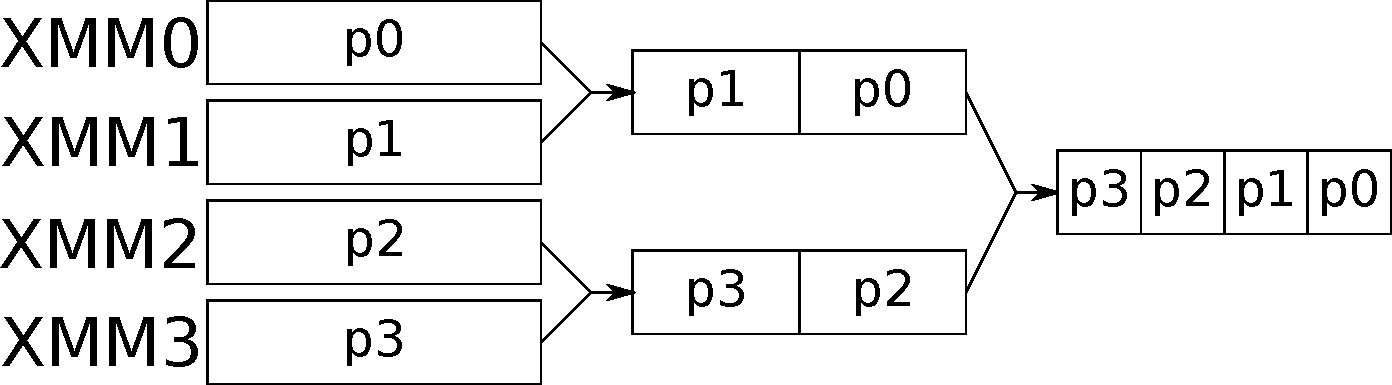
\includegraphics[scale=0.5]{images/MergeASM2_1}
\end{figure}

Al final tenemos:\\

\noindent
\texttt{XMM0 $\gets$ p3 * value $\vert$ p2 * value $\vert$ p1 * value $\vert$ p0 * value}\\
\texttt{XMM4 $\gets$ p3' * (1 - value) $\vert$ p2' * (1 - value) $\vert$ p1' * (1 - value) $\vert$ p0' * (1 - value)}\\

Para terminar solo fue necesario sumarlos y moverlos a memoria.

\subsection{Resultados}


% Para la experimentacion vamos a correr las 3 implementaciones (La version de $C$ compilada con optimizaciones de nivel 3) con la imagen de $lena$ brindada por la catedra (multiplos de 16x16, hasta 320x320), se corren 100 veces cada tamaño y despues se saca un promedio y se grafica el maximo, el minimo y el promedio.

% \begin{figure}[h!]
% 	\centering
% 	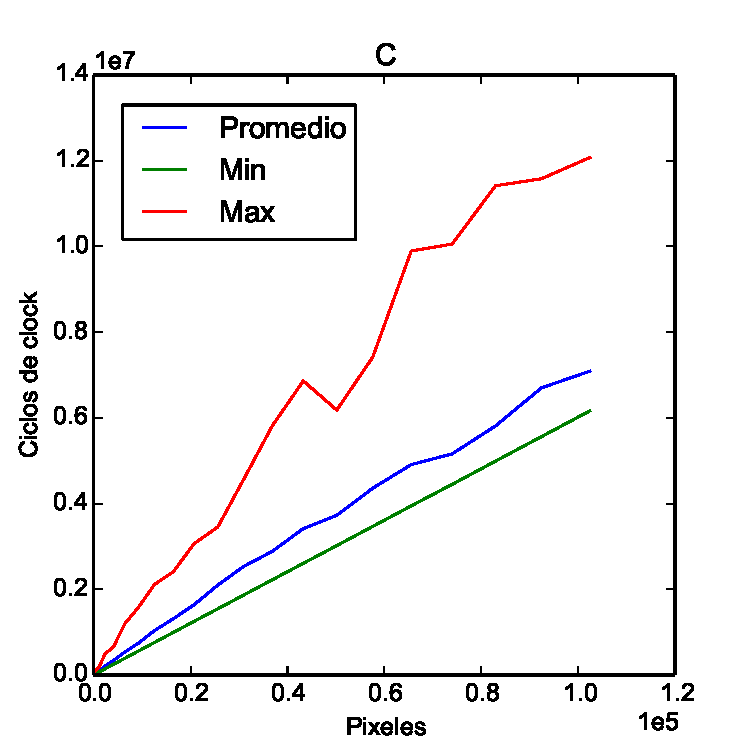
\includegraphics[scale=0.45]{images/c_merge}
% 	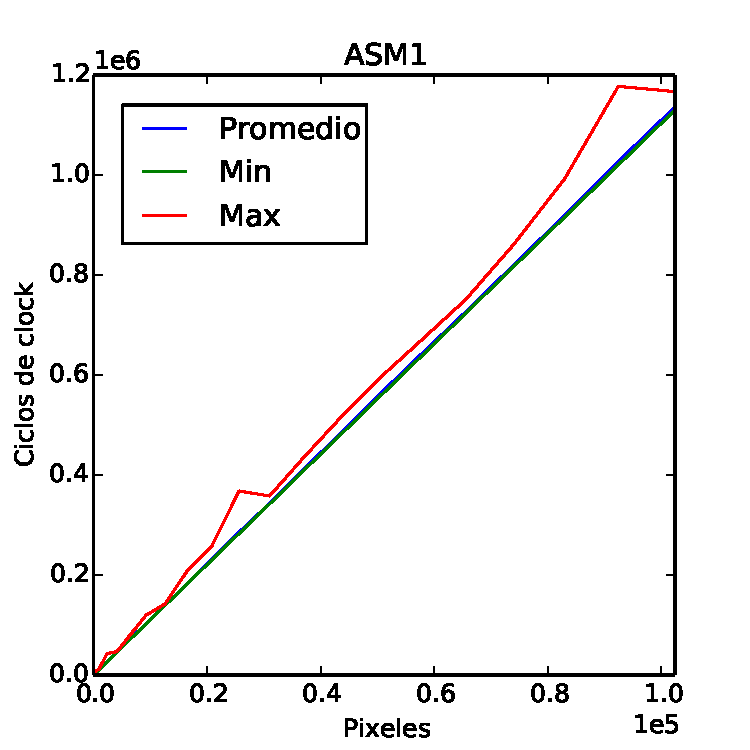
\includegraphics[scale=0.45]{images/asm1_merge}
% 	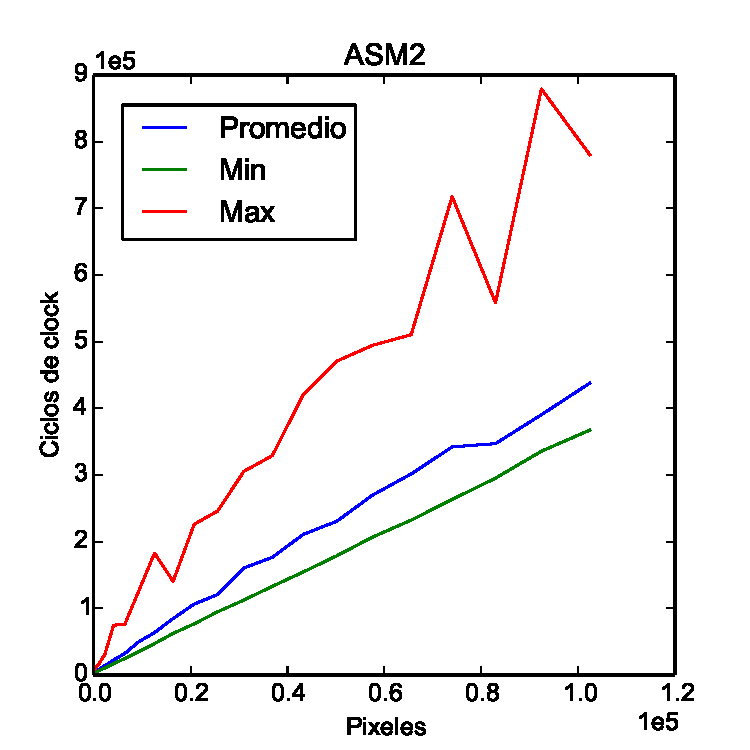
\includegraphics[scale=0.45]{images/asm2_merge}
% \end{figure}

% Tambien graficamos los 3 promedios en un grafico para ver cual de ellos es el mas rapido en general. Y para ver mejor la diferencia entre ASM1 y ASM2 los graficamos aparte.

% \begin{figure}[h!]
% 	\centering
% 	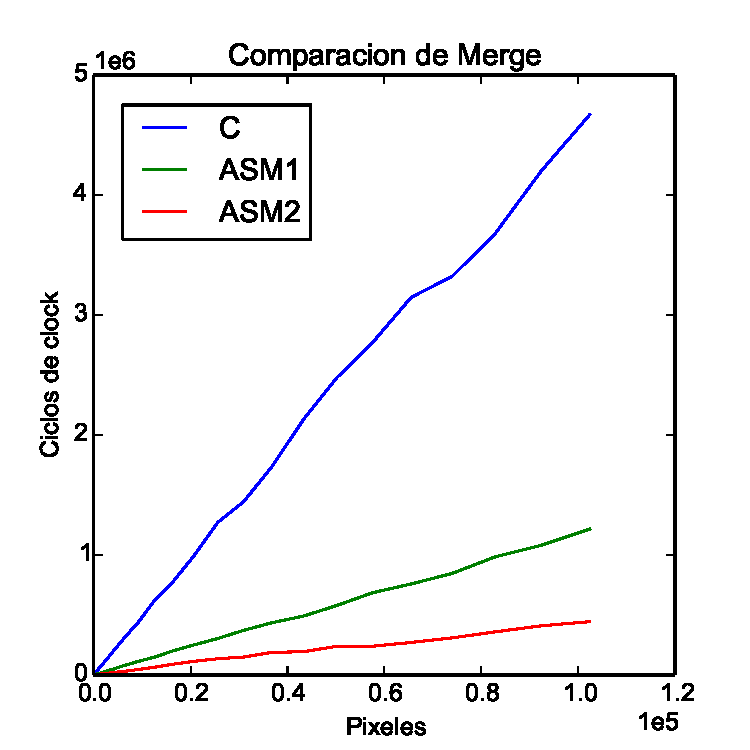
\includegraphics[scale=0.5]{images/c_asm1_asm2_merge_comp}
% 	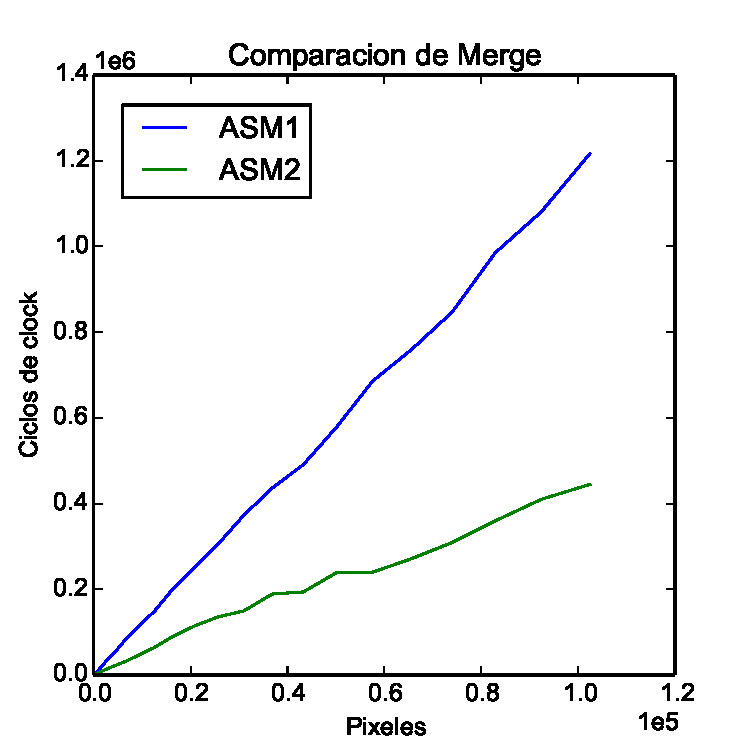
\includegraphics[scale=0.5]{images/asm1_asm2_merge_comp}
% \end{figure}
% \newpage

% Tambien queremos ver que la imagen no modifique el tiempo de ejecucion, tanto el codigo de C como el de ASM no poseen ningun salto condicional que depende de el valor de los pixeles.

% \begin{figure}[h!]
% 	\centering
% 	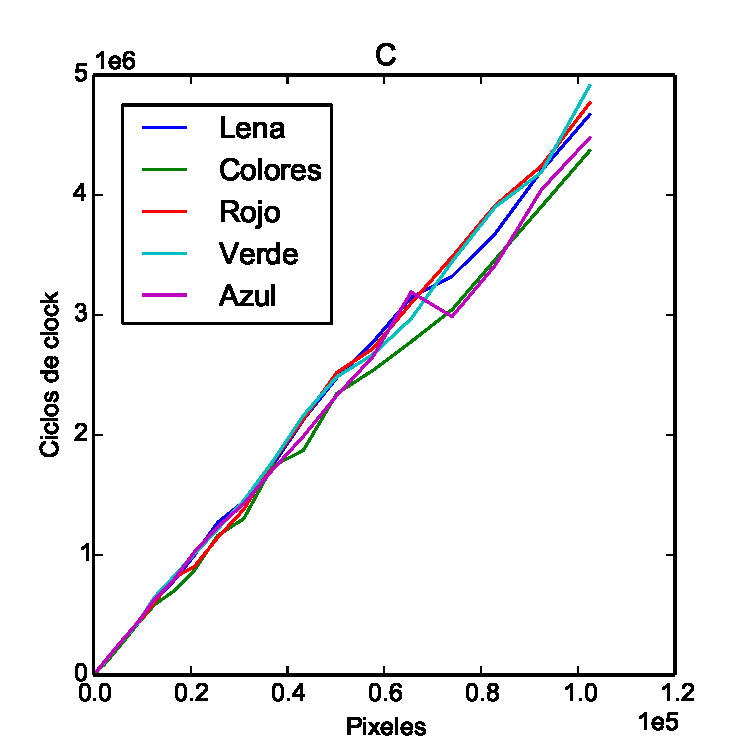
\includegraphics[scale=0.45]{images/c_merge_lena_colors}
% 	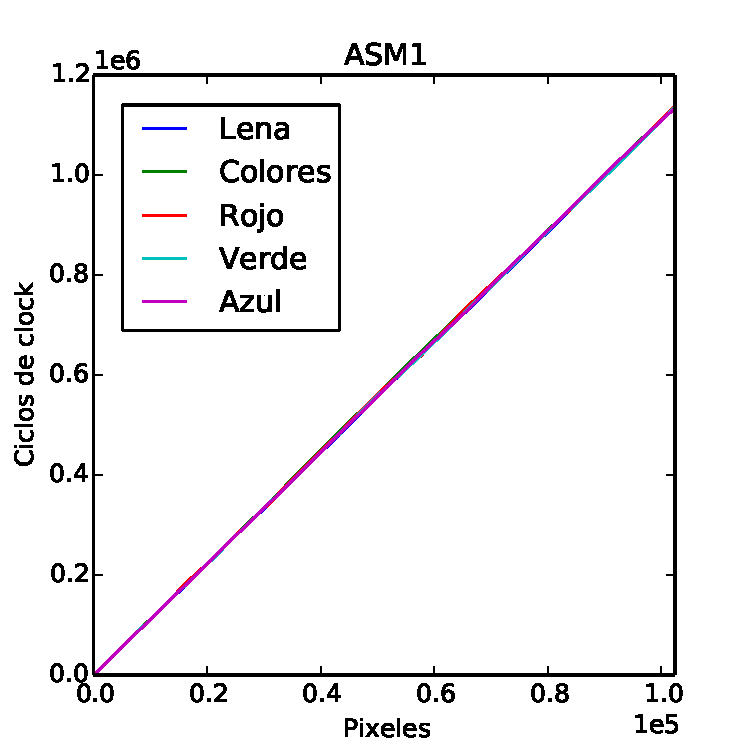
\includegraphics[scale=0.45]{images/asm1_merge_lena_colors}
% 	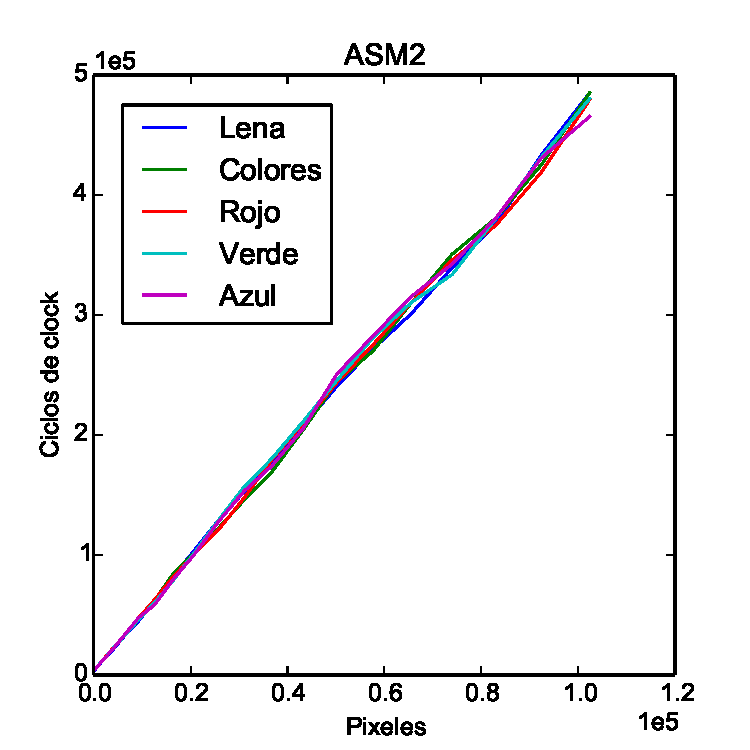
\includegraphics[scale=0.45]{images/asm2_merge_lena_colors}
% \end{figure}

\subsection{Conclusion}


% Al igual que en el primer filtro, las implementacion de $Assembler$ terminaron siendo mas veloces que la de $C$. La consistencia de los resultados tambien nos lleva a concluir que el costo en tiempo de hacer las conversiones en la primer implementacion es considerable, ya que la segunda version, al estar realizada sobre enteros minimizando las operaciones de punto flotante, tardo considerablemente menos.
\newpage

\section{Filtro 3: HSL}

\subsection{Explicacion}

La idea de este filtro consiste en transformar una imagen del espacio RGB a HSL, sumarle un valor recibido por parametro a cada una de las componentes y luego convertir la imagen de HSL a RGB, esto debe hacerse sobre la totalidad de los pixeles. Para las conversiones de espacio y la suma, la catedra proveyo las ecuaciones apropiadas junto con una implementacion en $C$ de las tres etapas.

\subsection{Implementacion 1}

Para la primer implementacion habia que implementar unicamente la etapa de $suma$ en $Assembler$, utilizando las funciones de $C$ provistas por la catedra para la conversion de RGB a HSL y viceversa. La ecuaciones de $suma$ son las siguientes:

\begin{align*}
suma_h(h, HH) =
\begin{cases}
h + HH - 360 &\mbox{si}\ h + HH \geq 360\\
h + HH + 360 &\mbox{si}\ h + HH < 0     \\
h + HH
\end{cases}
\\
suma_s(s, SS) =
\begin{cases}
1 &\mbox{si}\ s + SS \geq 1\hspace{17mm}\\
0 &\mbox{si}\ s + SS < 0   \\
s + SS
\end{cases}
\\
suma_l(l, LL) =
\begin{cases}
1 &\mbox{si}\ l + LL \geq 1\hspace{18mm}\\
0 &\mbox{si}\ l + LL < 0   \\
l + LL
\end{cases}
\end{align*}

Para las operaciones con punto flotante se empleo el tipo $float$. Para comenzar las operaciones de $suma$, partimos de los siguientes registros \texttt{XMM} con sus respectivos valores:\\

\noindent
\texttt{XMM0 $\gets$   LL  $\vert$   SS  $\vert$   HH  $\vert$ - }\\
\texttt{XMM1 $\gets\ $   l  $\vert\ $   s  $\vert\ $   h  $\vert$ - }\\

Tambien se cargaron en las siguientes mascaras:\\

\noindent
\texttt{XMM2 $\gets$  1.0  $\vert$  1.0  $\vert\ $  0.0  $\ \vert$ - }\\
\texttt{XMM3 $\gets$  0.0  $\vert$  0.0  $\vert\ $  0.0  $\ \vert$ - }\\
\texttt{XMM6 $\gets$  0.0  $\vert$  0.0  $\vert$  360.0  $\vert$ - }\\
\texttt{XMM7 $\gets$  0.0  $\vert$  0.0  $\vert\ $  0.0  $\ \vert$ - }\\
\texttt{XMM8 $\gets$  0.0  $\vert$  0.0  $\vert$  360.0  $\vert$ - }\\
\texttt{XMM9 $\gets$  0.0  $\vert$  0.0  $\vert$  360.0  $\vert$ - }\\

Con estos valores en los registros, se procedio a realizar la suma de la componentes de \texttt{XMM0} y \texttt{XMM1} con la instruccion \texttt{ADDPS} guardando el resultado en \texttt{XMM0}, y luego se almcenaron dos copias del mismo en \texttt{XMM4} y \texttt{XMM5} mediante la instruccion \texttt{MOVDQU}

La copia de \texttt{XMM4} se utilizo junto con las mascaras \texttt{XMM2} y \texttt{XMM3}, para poder satisfacer $suma_s$ y $suma_l$. Primero se tomo el minimo entre \texttt{XMM4} y \texttt{XMM2}, almacenando el resultado en \texttt{XMM4}, luego se procedio a tomar el maximo entre \texttt{XMM4} y \texttt{XMM3}, nuevamente guardando el resultado en \texttt{XMM4}. Esto nos sirve para respetar la funcion de $suma_s$ y $suma_l$, ya que en caso de que nuestros valores de $s$ o $l$ se excedan de \texttt{1.0}, el mismo pasaria a ser \texttt{1.0}, el mismo razonamiento aplica en el caso de que alguna de esas dos componentes sea menor a \texttt{0.0}.
\newpage
Una vez que tenemos los valores correspondientes en \texttt{XMM4}, procedemos a hacer un shuffle con el registro XMM0. El mismo lo hacemos con la instruccion \textsc{SHUFPS}, este responde al comportamiento mostrado en el siguiente grafico:

\begin{figure}[!h]
	\centering
	\includegraphics[scale=1.25]{images/HSLASM1_0}
\end{figure}

Con los valores correctos de $s + SS$ y $l + LL$, solo queda analizar $h + HH$. Para hacer esto empleamos las mascaras de \texttt{XMM6} y \texttt{XMM7}, procedimos a hacer una comparacion entre estas y el registro \texttt{XMM5} para obtener las nuevas mascaras que nos permitieron filtrar los condicionales de $suma_h$. La secuencia de operaciones fue la siguiente:\\

\noindent
\texttt{XMM6 $\gets$ XMM5 $\geq$ 360.0} \\
\texttt{XMM7 $\gets$ XMM5 $\geq$ 0} \\
\texttt{XMM6 $\gets$ XMM5 AND XMM8} \\
\texttt{XMM7 $\gets$ NOT(XMM7) AND XMM9} \\

Para las comparaciones se utilizo \texttt{CMPPS} y para las ultimas dos se utilizo \texttt{ANDPS} y \textsc{ANDNPS} respectivamente. Una vez finalizadas estas operaciones, si $h + HH$ se excede o iguala a \texttt{360.0}, en el tercer float de \texttt{XMM6} tendriamos el valor \texttt{360.0} mientras que en el caso que $h + HH$ sea menor a \texttt{0.0}, tendriamos el valor \texttt{360.0} en el tercer float de \texttt{XMM7}, si no se cumplen esas condiciones tendriamos el valor \texttt{0.0} en el tercer float del registro que no haya cumplido con el condicional. Con estos valores, lo unica operacion faltante fue a \texttt{XMM0} restarle \texttt{XMM6}, a este luego sumarle \texttt{XMM7} y guardar el resultado en \texttt{XMM0}, esto nos permite satisfacer el condicional de $suma_h$, y como originalmente \texttt{XMM6} y \texttt{XMM7} tenia \texttt{0.0} en los primeros dos $float$, esto hace que la ultima suma y resta no afecte los valores de $s$ y $l$, ya que tanto \texttt{XMM6} y \texttt{XMM7} siguen teniendo \texttt{0.0} en los primeros dos $float$. Teniendo en cuenta esto, tenemos finalmente en \texttt{XMM0} un registro que cumple con:\\

\noindent
\texttt{XMM0 $\gets$} $suma_l(l,LL)$ $\vert$ $suma_s(s,SS)$ $\vert$ $suma_h(h,HH)$ $\vert$ - \\

Con esto concluimos la etapa $suma$ de la primer implementacion, solo resta llamar a la funcion $HSLtoRGB$ provista por la catedra y volcar el resultado de la conversion en memoria.

\subsection{Implementacion 2}

Para la segunda implementacion se nos pidio implementar las 3 etapas del filtro en $Assembler$. Para la etapa $suma$ se utilizo la misma implementacion que la primera.

\subsubsection{RGB a HSL}

Al igual que el caso de $suma$, la catedra proveyo de las ecuaciones apropiadas. Las mismas estan presentadas a continuacion:

\begin{align*}
h(r, g, b) =
\begin{cases}
0 &\mbox{si}\ cmax = cmin\\
60* (g-b)/d + 6 &\mbox{si}\ cmax = r \\
60* (b-r)/d + 2 &\mbox{si}\ cmax = g \\
60* (r-g)/d + 4 &\mbox{si}\ cmax = b 
\end{cases}
\pmod{360}\hspace{17mm}
\\
l(r, g, b) = \frac{cmax + cmin}{510}\hspace{73mm}
\\
s(r, g, b) =
\begin{cases}
0 &\mbox{si}\ cmax = cmin \\
(d/(1-\texttt{fabs}(2*l(r, g, b) - 1)))/255.0001
\end{cases}
\end{align*}

Donde $cmax = max(r,g,b)$, $cmin = min(r,g,b)$ y $d = cmax - cmin$.

\paragraph{Calculo de \texttt{h}\newline}

Primero procedimos a levantar las componentes del pixel de la memoria y copiarlo al registro \texttt{XMM1}, dicha operacion la hicimos con la instruccion \texttt{MOVD}. Despues desempaquetamos los datos de tipo $uint8$ a $int$, esto fue hecho mediante \texttt{PUNPCKLBW} y \texttt{PUNPCKLWD} en ese orden, aplicando las instruccion sobre \texttt{XMM1} junto con algun registro \texttt{XMM} que contenga \texttt{0} en todos sus bits. Una vez con los valores en su tamaño correspondiente, procedimos a calcular \texttt{cmax} y \texttt{cmin}, esto lo logramos utilizando tres copias de \texttt{XMM1}, aplicando shifts a dos de ellas y tomando el minimo y maximo vertical almacenando el resultado en \texttt{XMM5} y \texttt{XMM6} respectivamente, los shifts fueron logrados mediante las instrucciones \texttt{PSRLDQ} y \texttt{PSLLDQ} segun el sentido en el cual deseemos shiftear. Hasta este momento tenemos en los registros:\\

\noindent
\texttt{XMM0 $\gets\ $ B $\ \ \vert$ G $\vert$ R $\vert$ A}\\
\texttt{XMM1 $\gets\ $ B $\ \ \vert$ G $\vert$ R $\vert$ 0}\\
\texttt{XMM5 $\gets$ cmin    $\vert$ - $\vert$ - $\vert$ -}\\
\texttt{XMM6 $\gets$ cmax    $\vert$ - $\vert$ - $\vert$ -}\\

El registro \texttt{XMM0} contiene una copia con el canal $alpha$ preservado, esta sera utilizada unicamente al final de la conversion.
Con \texttt{cmin} y \texttt{cmax} en sus respectivos registros, procedimos a limpiarlos con una mascara y a hacer un shuffle con \texttt{XMM6}, copiando la componente \texttt{cmax} en las cuatro componentes de \texttt{XMM2}. Luego, hicimos una nueva copia de \texttt{XMM1} en \texttt{XMM3} y mediante un shift y un \texttt{OR} con \texttt{XMM5}, logramos juntar las componentes \texttt{cmin}, \texttt{R}, \texttt{G} y \texttt{B} en un solo registro. Entonces tenemos:\\

\noindent
\texttt{XMM5 $\gets$ cmin $\vert\ $ 0 $\ \ \vert\ $ 0  $\ \ \vert\ $ 0}\\
\texttt{XMM6 $\gets$ cmax $\vert\ $ 0 $\ \ \vert\ $ 0  $\ \ \vert\ $ 0}\\
\texttt{XMM2 $\gets$ cmax $\vert$ cmax    $\vert$ cmax $\vert$ cmax}\\
\texttt{XMM3 $\gets$ cmin $\vert\ $ B $\ \ \vert\ $ G  $\ \ \vert\ $ R}\\

Los registros \texttt{XMM2} y \texttt{XMM3} fueron empleados para obtener la mascara para poder calcular la funcion $h(r,g,b)$. La misma fue obtenida utilizando la instruccion \texttt{PCMPEQD} entre \texttt{XMM3} y \texttt{XMM2}, almacenando el resultado de la comparacion de igualdad en \texttt{XMM3}. Una vez obtenida esta mascara, la misma fue reordenada via un shuffle, para seguir el mismo orden que el condicional de la implementacion $C$, el nuevo orden fue guardado en el registo \texttt{XMM4}. En esta etapa tenemos:\\

\noindent
\texttt{XMM3 $\gets$ cmin == cmax $\vert$ B == cmax $\vert$ G == cmax  $\vert\ \ \ $ R == cmax}\\
\texttt{XMM4 $\gets\ \ \ $ R == cmax $\vert$ G == cmax $\vert$ B == cmax  $\vert$ cmin == cmax}\\

Uno de los problemas encontrados durante la implementacion fueron los casos donde existian 2 o mas componentes que eran iguales a \texttt{cmax}, esto hacia que la mascara tuviese mas de una componente con \texttt{0xFFFFFFFF}, lo cual hacia que los resultados al filtrar fuesen incorrectos. Para solucionar esto propusimos armar una mascara, la cual tuviese \texttt{0xFFFFFFFF} en las componentes despues la primer componente distinta de cero de \texttt{XMM4}, lo unico necesario seria hacer \texttt{XOR} bit a bit entre la nueva mascara y \texttt{XMM4}. El grafico a continuacion ilustra la idea:

\begin{figure}[!h]
	\centering
	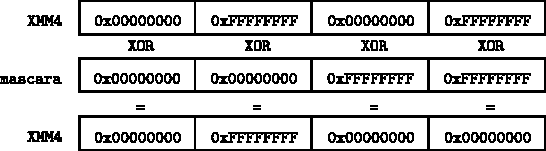
\includegraphics[scale=1.25]{images/HSLASM1_1}
\end{figure}

Una vez que tenemos esta mascara, preparamos los registros \texttt{XMM7}, \texttt{XMM8}, \texttt{XMM9} y \texttt{XMM11} con los siguientes valores y tambien disponiamos de una seria de constantes en memoria. Los valores de los registros y constantes son los siguientes:

\noindent
\texttt{XMM7  $\ \ \ \ \gets\ $ g $\ \ \vert\ $ b $\ \ \vert\ $ r  $\ \ \vert\ $ 0}\\
\texttt{XMM8  $\ \ \ \ \gets\ $ b $\ \ \vert\ $ r $\ \ \vert\ $ g  $\ \ \vert\ $ 0}\\
\texttt{XMM9  $\ \ \ \ \gets$ cmax $\vert$ cmax    $\vert$ cmax $\vert$ cmax}\\
\texttt{XMM11 $\ \ \ \gets$ cmin $\vert$ cmin    $\vert$ cmin $\vert$ cmin}\\
\texttt{cte\char`_suma $\gets\ $ 6.0 $\vert\ $ 2.0 $\vert\ $ 4.0 $\vert\ $ 0.0}\\
\texttt{cte\char`_60 $\ \ \gets$ 60.0 $\vert$ 60.0 $\vert$ 60.0 $\vert$ 60.0}\\

Se procedio a realizar las operaciones verticales apropiadas para poder satisfacer la funcion $h(r,g,b)$. La unica salvedad es que luego de efectuar las operaciones de resta entre \texttt{XMM7} y \texttt{XMM8}, y la de \texttt{XMM11} y \texttt{XMM9}, el resultado de ambas fue convertido a $float$ mediante la instruccion \texttt{CVTDQ2PS} y almcenado en los registros \texttt{XMM8} y \texttt{XMM10} respectivamente. Posteriormente se procedio con el resto de las operaciones con las instrucciones de punto flotante apropiadas, y se guardo el resultado en \texttt{XMM8}, a este luego se le aplico la mascara guardada en \texttt{XMM4}.

Otro problema que encontramos fue el caso \texttt{cmin == cmax}, aqui tenemos que \texttt{d} es igual a cero, con lo cual al proceder con las divisiones nos topariamos con un NaN, para solucionar esto decidimos armar una nueva mascara que contenga \texttt{cmin == cmax} en cada una de sus componentes. Para hacerlo alcanzo con utilizar el registro \texttt{XMM9} y \texttt{XMM2} (el mismo no fue modificado y mantiene los mismos valores que arriba) para hacer la comparacion de igualdad, el resultado de la misma fue guardado en \texttt{XMM9}. Con esto se procedio a hacer la operacion \texttt{NOT(XMM9) AND XMM8}, y para poder calcular el mód 360 de $h(r,g,b)$ se aplico la misma logica que en caso de $suma$ ya que los calculos para $h$ no van a excederse de 720. Finalmente tenemos en \texttt{XMM10}:\\

\noindent
\texttt{XMM10  $\gets$ - $\vert$ - $\vert$ - $\vert$ h}\\

\paragraph{Calculo de \texttt{l} y \texttt{s}\newline}

Para el calculo de \texttt{l} no hubo ninguna particularidad, el mismo se hizo en base a los siguientes registros y constantes:\\

\noindent
\texttt{XMM7 $\ \ \ \gets\ $ cmax $\vert\ \ $ 0 $\ \ \vert\ \ $ 0 $\ \ \vert\ \ $ 0}\\
\texttt{XMM5 $\ \ \ \gets\ $ cmin $\vert\ \ $ 0 $\ \ \vert\ \ $ 0 $\ \ \vert\ \ $ 0}\\
\texttt{cte\char`_510  $\gets$ 510.0 $\vert$ 510.0 $\vert$ 510.0 $\vert$ 510.0}\\

Primero se realizo la resta entre \texttt{XMM7} y \texttt{XMM5} almacenando el resultado en \texttt{XMM7}, a esta se la convirtio a $float$ mediante \texttt{CVTDQ2PS} previo a la multiplicacion con \texttt{cte\char`_510}. Tenemos finalmente en resultado en \texttt{XMM8}, el mismo tiene la pinta:\\

\noindent
\texttt{XMM8  $\gets$ l $\vert$ 0 $\vert$ 0 $\vert$ 0}\\

Para el calculo de \texttt{s} se utilizaron los siguientes registros, mascaras y constantes:\\

\noindent
\texttt{XMM7 $\ \ \ \ \ \ \ \gets\ \ \ $ cmax $\ \ \ \vert\ $ 0 $\ \vert\ $ 0 $\ \vert\ $ 0}\\
\texttt{XMM5 $\ \ \ \ \ \ \ \gets\ \ \ $ cmin $\ \ \ \vert\ $ 0 $\ \vert\ $ 0 $\ \vert\ $ 0}\\
\texttt{XMM5 $\ \ \ \ \ \ \ \gets\ \ \ \ $ l $\ \ \ \ \ \vert\ $ 0 $\ \vert\ $ 0 $\ \vert\ $ 0}\\
\texttt{cte\char`_1  $\ \ \ \ \ \ \gets\ \ \ $ 1.0 $\ \ \ \ \vert$ 1.0 $\vert$ 1.0 $\vert$ 1.0}\\
\texttt{cte\char`_2  $\ \ \ \ \ \ \gets\ \ \ $ 2.0 $\ \ \ \ \vert$ 2.0 $\vert$ 2.0 $\vert$ 2.0}\\
\texttt{cte\char`_255  $\ \ \ \ \gets\ $ 255.0001 $\ \vert\ $ 0 $\ \vert\ $ 0 $\ \vert\ $ 0}\\
\texttt{masc\char`_abs  $\ \ \ \gets$ 0x7FFFFFFF $\vert\ $ 0 $\ \vert\ $ 0 $\ \vert\ $ 0}\\
\texttt{limpiar\char`_msb  $\gets$ 0xFFFFFFFF $\vert\ $ 0 $\ \vert\ $ 0 $\ \vert\ $ 0}\\

En este caso hay dos puntos a destacar, estos son el condicional de $s(r,g,b)$ y el \texttt{fabs}. Para poder filtrar segun si \texttt{cmax == cmin} alcanza con hacer una comparacion de igualdad entre \texttt{cmax} y \texttt{cmin} mediante \texttt{PCMPEQD}, guardar el resultado de la misma en un registro, y luego de hacer las operaciones correspondientes aplicar el resultado de la comparacion mediante un \texttt{AND}. En el caso del \texttt{fabs}, al estar operando con numeros de tipo $float$ codificados bajo la norma IEEE 754, basta con colocar el bit mas significativo en cero, esto lo podemos hacer mediante un \texttt{AND} con el numero al cual deseamos aplicar \texttt{fabs} y la \texttt{masc\char`_abs}. Finalmente tenemos en el registro \texttt{XMM7}:\\

\noindent
\texttt{XMM7 $\gets$ s $\vert$ 0 $\vert$ 0 $\vert$ 0}\\

Con los valores de \texttt{h}, \texttt{s} y \texttt{l} calculados, lo unico que falta por hacer es juntar todo en un solo registro junto con el dato del canal $alpha$, el cual se encuentra en el registro \texttt{XMM0}. Para hacer esto, vamos a shiftear los registros que contienen a \texttt{s} y a \texttt{h}, 4 y 8 bytes hacia la derecha respectivamente. Una vez que tenemos esto, lo vamos a juntar a todos en un unico registro mediante un \texttt{OR} y vamos a procede a aplicarle a \texttt{XMM0} la mascara \texttt{limpiar\char`_msb}, convertir el resultado a $float$ y juntarlo junto con lo que ya teniamos utilizando nuevamente un \texttt{OR}. Con esto podemos concluir la etapa $RGBtoHSL$.

\subsubsection{HSL a RGB}

Tanto como en el caso de $suma$ y $RGBtoHSL$, la catedra proveyo las ecuaciones necesarias para la conversion, las mismas son:\\

\begin{align*}
RGBAux(h, s, l) =
\begin{cases}
(c,x,0) &\mbox{si}\ 0 \leq h < 60\\
(x,c,0) &\mbox{si}\ 60 \leq h < 120\\
(0,c,x) &\mbox{si}\ 120 \leq h < 180\\
(0,x,c) &\mbox{si}\ 180 \leq h < 240\\
(x,0,c) &\mbox{si}\ 240 \leq h < 300\\
(c,0,x) &\mbox{si}\ 300 \leq h < 360
\end{cases}
\hspace{62mm}
\\
RGB(h,s,l) = (RGBAux(h,s,l)_r * 255, RGBAux(h,s,l)_g * 255, RGBAux(h,s,l)_b * 255)
\end{align*}

Donde $c = (1 - fabs(2*l - 1))*s$, $x = c*(1 - fabs(fmod(h/60, 2) - 1))$ y $m = 1 - c/2$. Se tuvo que hacer un cambio, ya que en el enunciado las componentes \texttt{B} y \texttt{G} se encontraban invertidas, imposibilitando la conversion correcta.

Para poder hacer el calculo de \texttt{R}, \texttt{G}, \texttt{B} tuvimos que hacer el de \texttt{c}, \texttt{x} y \texttt{m}.

\paragraph{Calculo de \texttt{c}\newline}

Para el calculo de \texttt{c}, tenemos los siguientes registros, mascaras y constantes:\\

\noindent
\texttt{XMM1 $\ \ \ \ \gets \ \ \ \ $ l $\ \ \ \ \ \vert\ \ \ \ $ l $\ \ \ \ \ \vert\ \ \ \ $ l  $\ \ \ \ \ \vert\ \ \ \ $ l}\\
\texttt{XMMn $\ \ \ \ \gets \ \ \ \ $ s $\ \ \ \ \ \vert\ \ \ \ $ s $\ \ \ \ \ \vert\ \ \ \ $ s  $\ \ \ \ \ \vert\ \ \ \ $ s}\\
\texttt{cte\char`_1 $\ \ \ \gets\ \ \ $ 1.0 $\ \ \ \ \vert\ \ \ $ 1.0 $\ \ \ \ \vert\ \ \ $ 1.0 $\ \ \ \ \vert\ \ \ $ 1.0}\\
\texttt{cte\char`_2 $\ \ \ \gets\ \ \ $ 2.0 $\ \ \ \ \vert\ \ \ $ 2.0 $\ \ \ \ \vert\ \ \ $ 2.0 $\ \ \ \ \vert \ \ \ $ 2.0}\\
\texttt{masc\char`_abs $\gets$ 0x7FFFFFFF $\vert$ 0x7FFFFFFF $\vert$ 0x7FFFFFFF $\vert$ 0x7FFFFFFF}\\

Con estos podemos hacer las operaciones correspondientes para satisfacer el calculo de \texttt{c}. El unico caso que requiere atencion particular es el de \texttt{fabs}, debido a que los numeros de punto flotante estan codificados con la norma IEEE 754, lo unico que hace falta para poder obtener el valor absoluto es colocar el bit mas significativo de cada $float$ en cero, para hacer esto alcanza con aplicar la mascara \texttt{masc\char`_abs} mediante la instruccion \texttt{ANDPS} al registro apropiado. Tras finalizar las operaciones tenemos en \texttt{XMM1}:\\

\noindent
\texttt{XMM1 $\gets$ c $\vert$ c $\vert$ c $\vert$ c}\\

Posteriormente procedimos a limpiar el registro, dejando unicamente el $float$ de las posicion menos significativa. Entonces obtenemos:\\

\noindent
\texttt{XMM1 $\gets$ 0 $\vert$ 0 $\vert$ 0 $\vert$ c}\\

Esto lo hacemos para despues poder armar todas las posiblidades de $RGBAux(h,s,l)$.

\paragraph{Calculo de \texttt{x}\newline}

Al igual que con \texttt{c}, vamos a empezar por los registros:\\

\noindent
\texttt{XMM0 $\ \ \ \ \gets \ \ \ \ $ l $\ \ \ \ \ \vert\ \ \ \ $ s $\ \ \ \ \ \vert\ \ \ \ $ h  $\ \ \ \ \ \vert\ \ \ \ $ a}\\
\texttt{XMM1 $\ \ \ \ \gets \ \ \ \ $ 0 $\ \ \ \ \ \vert\ \ \ \ $ 0 $\ \ \ \ \ \vert\ \ \ \ $ 0  $\ \ \ \ \ \vert\ \ \ \ $ c}\\
\texttt{XMM3 $\ \ \ \ \gets \ \ \ \ $ h $\ \ \ \ \ \vert\ \ \ \ $ h $\ \ \ \ \ \vert\ \ \ \ $ h  $\ \ \ \ \ \vert\ \ \ \ $ h}\\
\texttt{cte\char`_1 $\ \ \ \gets\ \ \ $ 1.0 $\ \ \ \ \vert\ \ \ $ 1.0 $\ \ \ \ \vert\ \ \ $ 1.0 $\ \ \ \ \vert\ \ \ $ 1.0}\\
\texttt{cte\char`_2 $\ \ \ \gets\ \ \ $ 2.0 $\ \ \ \ \vert\ \ \ $ 2.0 $\ \ \ \ \vert\ \ \ $ 2.0 $\ \ \ \ \vert \ \ \ $ 2.0}\\
\texttt{cte\char`_60 $\ \ \gets\ \ $ 60.0 $\ \ \ \ \vert\ \ $ 60.0 $\ \ \ \ \vert\ \ $ 60.0 $\ \ \ \ \vert \ \ $ 60.0}\\
\texttt{masc\char`_abs $\gets$ 0x7FFFFFFF $\vert$ 0x7FFFFFFF $\vert$ 0x7FFFFFFF $\vert$ 0x7FFFFFFF}\\

Con estos valores podemos hacer facilmente los calculos de \texttt{x}, para \texttt{fabs} aplicamos la misma logica que antes, el unico caso que requiere atencion particular es el de \texttt{fmod}. La funcion \texttt{fmod} realiza las siguientes operaciones:

$$
fmod(a, b) = a - \left\lfloor\frac{a}{b}\right\rfloor * b 
$$

Para poder implementar esta funcion con instrucciones SSE, tenemos que encontrar una forma de tomar la parte entera de la division, para hacer esto decidimos utilizar la instruccion \texttt{ROUNDPS}, la misma si es uilizada con el inmediato \texttt{0x03} nos permite guardar una version redondeada con cero en la parte decimal del operando fuente. Una vez que disponimos de este resultado, solo queda aplicar la multiplicacion y resta correspondiente.
Una vez finalizadas las operaciones requeridas, tenemos en \texttt{XMM2}:\\

\noindent
\texttt{XMM2 $\gets$ 0 $\vert$ 0 $\vert$ 0 $\vert$ x}\\

Los primeros tres $float$ quedan en cero puesto a que al hacer la multiplicacion con \texttt{XMM1}, el mismo tenia \texttt{c} unicamente en la ultima componente.

\paragraph{Calculo de \texttt{m}\newline}

Para el calculo de \texttt{m} no hubo mayor particularidad, el mismo se llevo a cabo con los siguientes registros y mascaras:\\

\noindent
\texttt{XMM3 $\ \gets$ l $\vert$ l $\vert$ l $\vert$ l}\\
\texttt{XMM4 $\ \gets$ c $\vert$ c $\vert$ c $\vert$ c}\\
\texttt{cte\char`_2 $\gets$ 2 $\vert$ 2 $\vert$ 2 $\vert$ 2}\\

El resultado final fue guardado en el registro \texttt{XMM3}, el mismo quedo asi:\\

\noindent
\texttt{XMM3 $\gets$ m $\vert$ m $\vert$ m $\vert$ m}\\

\paragraph{Calculo de RGB\newline}

Para el calculo de $RGBAux$, se tuvieron que armar seis mascaras, las mismas filtraban los 6 casos de la funcion. Para armarlas se conto con los siguientes registros y constantes:\\

\noindent
\texttt{XMM9 $\ \ \ \ \gets\ \ $ h $\ \ \vert\ \ $ h $\ \ \vert\ \ $ h $\ \ \vert\ \ $ h}\\
\texttt{cte\char`_cmp1 $\gets$ 180.0 $\vert$ 240.0 $\vert$ 300.0 $\vert$ 360.0}\\
\texttt{cte\char`_cmp2 $\gets$ 120.0 $\vert$ 180.0 $\vert$ 240.0 $\vert$ 300.0}\\
\texttt{cte\char`_cmp3 $\gets\ \ $ 0.0 $\vert\ \ $ 0.0 $\vert\ $ 60.0 $\vert$ 120.0}\\
\texttt{cte\char`_cmp4 $\gets\ \ $ 0.0 $\vert\ \ $ 0.0 $\vert\ \ $ 0.0 $\vert\ $ 60.0}\\

La idea consistio en comparar si \texttt{XMM9} $<$ cte\texttt{\char`_cmp1} y \texttt{XMM9} $\geq$ \texttt{cte\char`_cmp2}, luego se procedio a unificar estas dos comparaciones con un \texttt{AND}, es decir, nos quedamos unicamente con los casos donde una componente de \texttt{XMM9} sea menor a su respectiva componente de \texttt{cte\char`_cmp1} y mayor o igual a la de \texttt{cte\char`_cmp2}, luego se almaceno el resultado en \texttt{XMM10}. Este mismo proceso fue repetido pero con \texttt{cte\char`_cmp3} y \texttt{cte\char`_cmp4}, y el resultado fue almacenado en \texttt{XMM12}. Estos resultados luego fueron expandidos a 6 registros \texttt{XMM} mediante un shuffle, el proceso responde al siguiente grafico:\\

\begin{figure}[!h]
	\centering
	\includegraphics[scale=1.25]{images/HSLASM1_2}
\end{figure}

Con estas mascaras armadas, se procedio a armar las 6 posbiles combinaciones de \texttt{R}, \texttt{G} y \texttt{B}. Las mismas son:\\

\noindent
\texttt{XMM10 $\gets$ 0 $\vert$ x $\vert$ c $\vert$ 0}\\
\texttt{XMM11 $\gets$ 0 $\vert$ c $\vert$ x $\vert$ 0}\\
\texttt{XMM12 $\gets$ x $\vert$ c $\vert$ 0 $\vert$ 0}\\
\texttt{XMM13 $\gets$ c $\vert$ x $\vert$ 0 $\vert$ 0}\\
\texttt{XMM14 $\gets$ c $\vert$ 0 $\vert$ x $\vert$ 0}\\
\texttt{XMM15 $\gets$ x $\vert$ 0 $\vert$ c $\vert$ 0}\\

Lo unico restante fue aplicar cada una de las mascaras formadas anteriormente a su correspondiente registro de la lista anterior mediante un \texttt{AND}, y luego sumar todo en un solo registro. Con eso ya teniamos el valor final de $RGBAux$ en el registro \texttt{XMM4}, ademas de este teniamos tambien el siguientes registro y constante:\\

\noindent
\texttt{cte\char`_255 $\gets$ 255.0 $\vert$ 255.0 $\vert$ 255.0 $\vert$ 255.0}\\
\texttt{XMM3 $\ \ \ \gets\ \ $ m $\ \ \vert\ \ $ m $\ \ \vert\ \ $ m $\ \ \vert\ \ $ m}\\

Con estos registros, lo unico faltante fue realizar las operaciones aritmeticas indicadas en la funcion $RGB$, mencionada al comienzo del esta seccion, y unificar el resultado con el canal $alpha$ del registro \texttt{XMM0}. Para hacer esto alcanzo con quedarnos unicamente con la componente menos significtiva y juntarla mediante un \texttt{OR} con el resultado final de $RGB$. Esto nos da el resultado final de la conversion, el siguiente paso fue convertir los numeros de tipo $float$ de 32 bits a $uint$ de 8 bits, para hacer esto basto con convertir de $float$ a $int$ de 32 bits via la instruccion \texttt{CVTPS2DQ} y empaquetar el resultado de 32 bits a 8 bits mediante las instrucciones \texttt{PACKUSDW} y \texttt{PACKUSWB}, en ese orden. Una vez concluido el empaquetado, procedimos a volcar dicho resultado a la misma posicion de memoria a partir de la cual iniciamos el ciclo.

\newpage
\subsection{Resultados}
Al igual que con $blur$ y $merge$, decidimos emplear la misma metodologia para poder medir la eficiencia de las implementaciones. Los resultados obtenidos fueron:

\begin{figure}[h!]
	\centering
	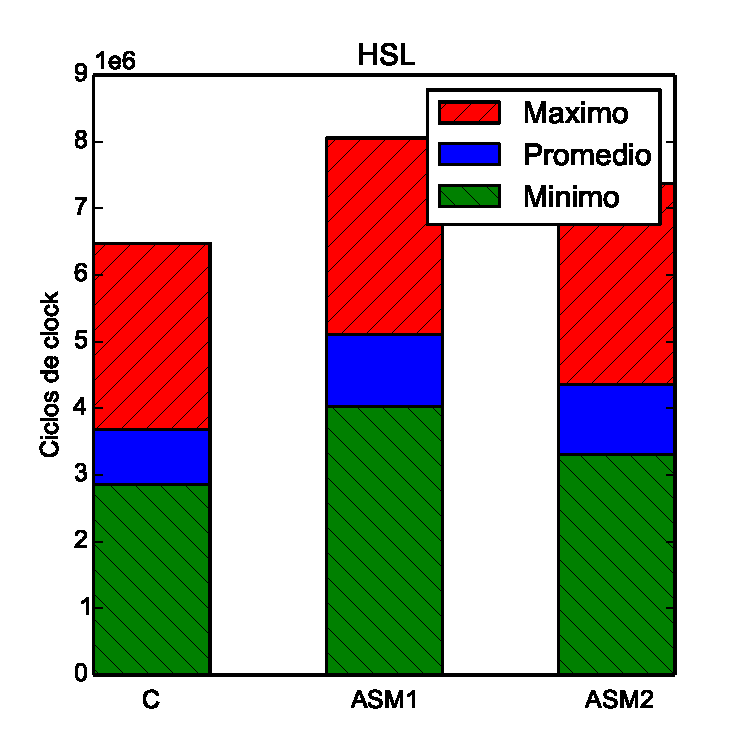
\includegraphics[scale=0.45]{images/hsl_comparation}
\end{figure}

Estos resultados nos sorprendieron ampliamente, despues de ver los de $blur$ y $merge$, pero estos tienen sentido. A diferencia de los otros filtros, este no se caracteriza por su linearidad ya que en las diferentes etapas del mismo se encuentran una gran cantidad de condicionales, esto nos obligo a tener una gran cantidad de mascaras y una aritmetica demasiado compleja aumentando el tiempo de ejecucion. Tampoco se pudo operar con mas de un pixel, ya que los condicionales podian dar resultados distintos para las diferentes componentes de cada pixel.

Como en este caso nos encontramos con condicionles que cambiaban el flujo del programa, decidimos realizar pruebas de rendimiento con las imagenes $lena$ y $colores$ provistas por la catedra (ambas de 160x160), y agregar 3 imagenes que tengan unicamente color rojo, verde y azul. Esto nos permite ver si los diferentes caminos en el flujo del codigo en $C$ afectan el rendimiento. Los resultados fueron:

\begin{figure}[h!]
	\centering
	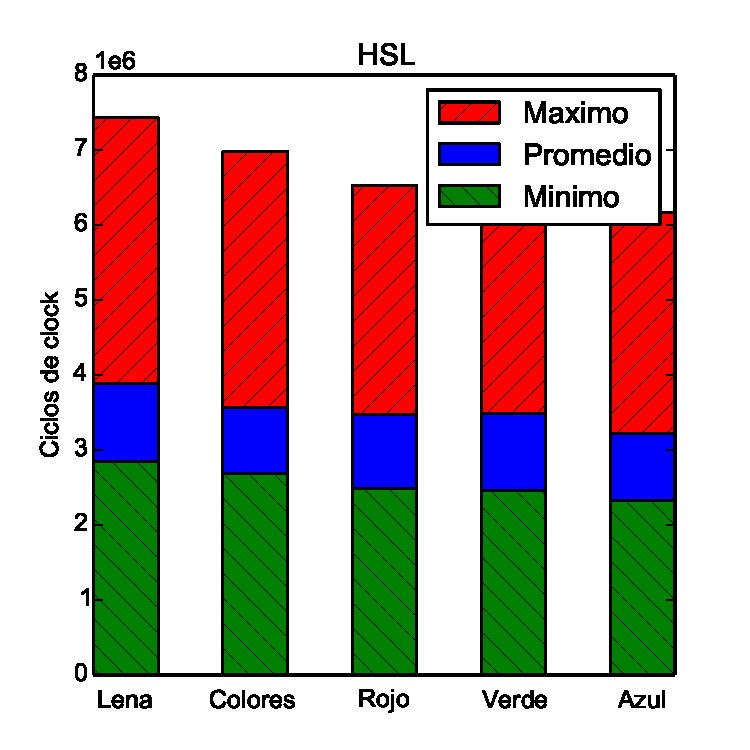
\includegraphics[scale=0.45]{images/hsl_comparationC}
	\caption{C}
\end{figure}

\newpage
\begin{figure}[h!]
	\centering
	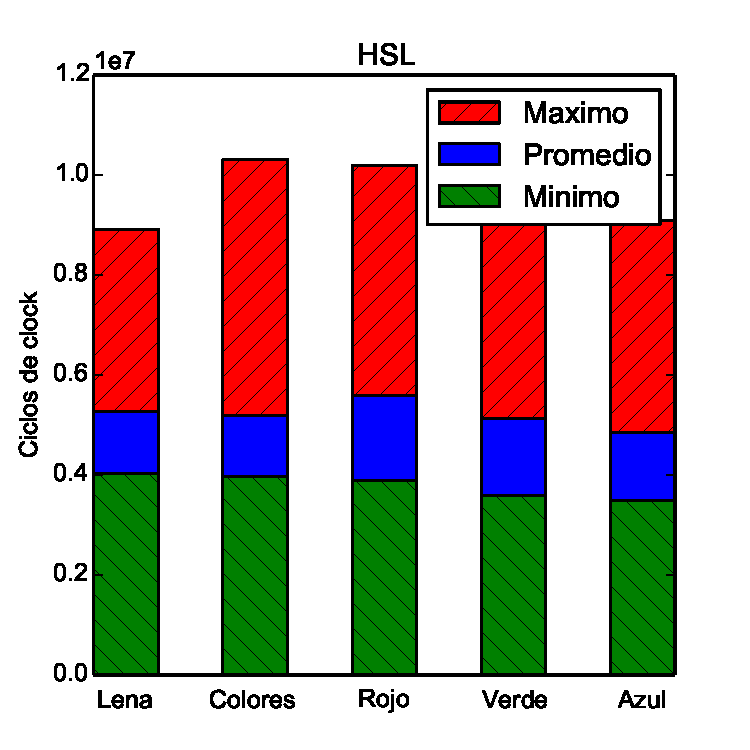
\includegraphics[scale=0.45]{images/hsl_comparationASM1}
	\caption{ASM1}
\end{figure}	

\begin{figure}[h!]
	\centering
	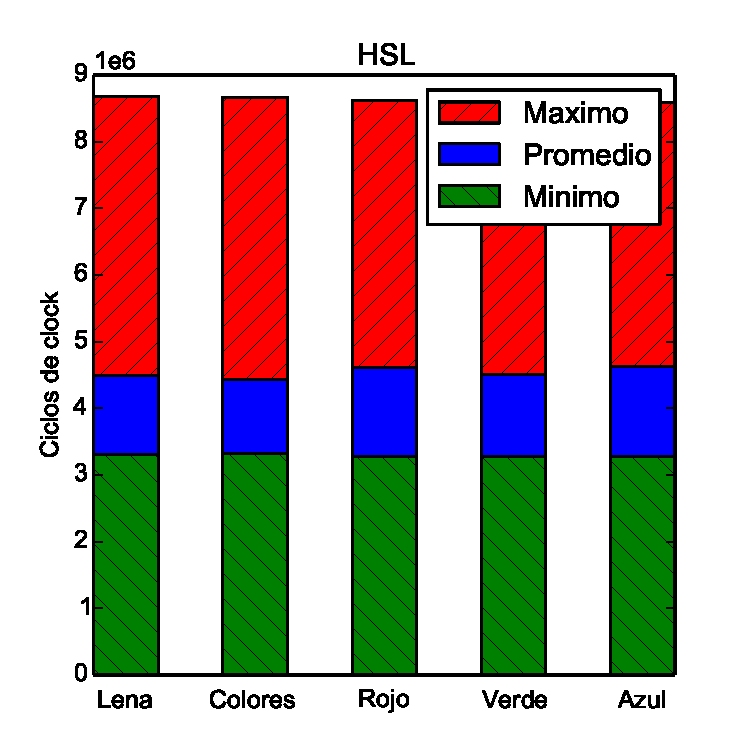
\includegraphics[scale=0.45]{images/hsl_comparationASM2}
	\caption{ASM2}
\end{figure}

Para la implementacion en $C$ no hubo mayor diferencia en la cantidad de ciclos que tomo cada imagen, en donde si hubo un mejor rendimiento fue en las imagenes que tienen un solo color, consideramos que esto se debe a que en este caso el flujo del programa es siempre el mismo para todos los pixeles.
Tambien se puede ver en las implementacion con SSE, que al tener menos saltos condicionales (o no tenerlos como es el caso de $ASM2$) el contenido de la imagen no impacta significativamente al rendimiento.

% Al igual que con los dos casos anteriores, empezamos corriendo la version de $C$ con optimizaciones de nivel 3, junto con la imagen $lena$ brindada por la catedra, se tomaron cien muestras con versiones de la imagen que fuesen multiplos de 16x16, hasta llegar a 320x320. Aqui se encuentran graficados el maximo, minimo y el promedio:\\

% \begin{figure}[h!]
% 	\centering
% 	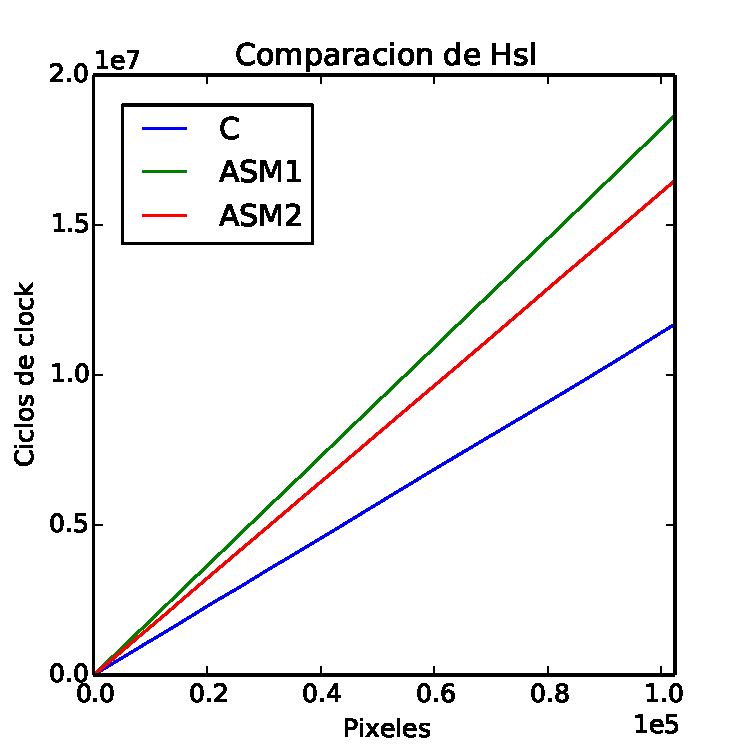
\includegraphics[scale=0.5]{images/c_asm1_asm2_hsl_comp}
% \end{figure}

% Los resultados fueron sorpresivos, ya que a diferencia de los dos filtros anteriores, aqui nos encontramos con que la version de $C$ era mas veloz que las implementaciones de $Assembler$. Esto nos llevo a plantearnos si los saltos condicionales de $C$ , en el peor caso, podian llegar a hacer que las implementaciones en $Assembler$ fuesen mas rapidas. Para probar eso se nos ocurrieron dos tests:\\

% \begin{itemize}
% 	\item Testear imagenes completamente rojas, azules y verdes (una de cada una), junto con $colores$ y $lena$, para ver si el salto condicional en $RGBtoHSL$ impactaba al rendimiento.
% 	\item Testear con diferentes valores de \texttt{HH}, tomando valores aleatorios entre cero y uno para \text{SS} y \texttt{LL}, esto lo hacemos para probar si el condicional de 6 casos en $HSLtoRGB$ afecta el rendimiento.
% \end{itemize}

% Para el primer test se obtuvieron los siguientes resultados:\\

% \begin{figure}[h!]
% 	\centering
% 	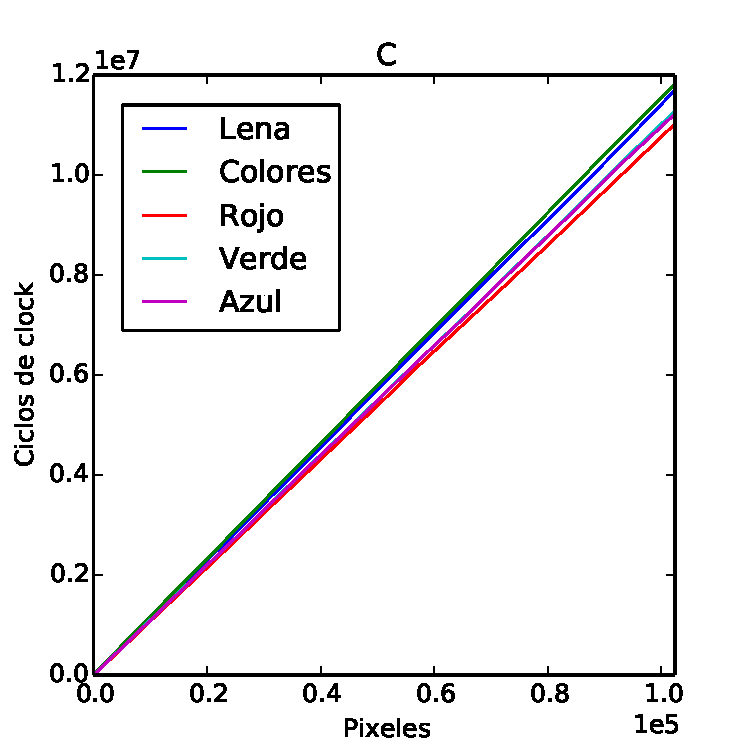
\includegraphics[scale=0.45]{images/c_hsl_lena_colors}
% 	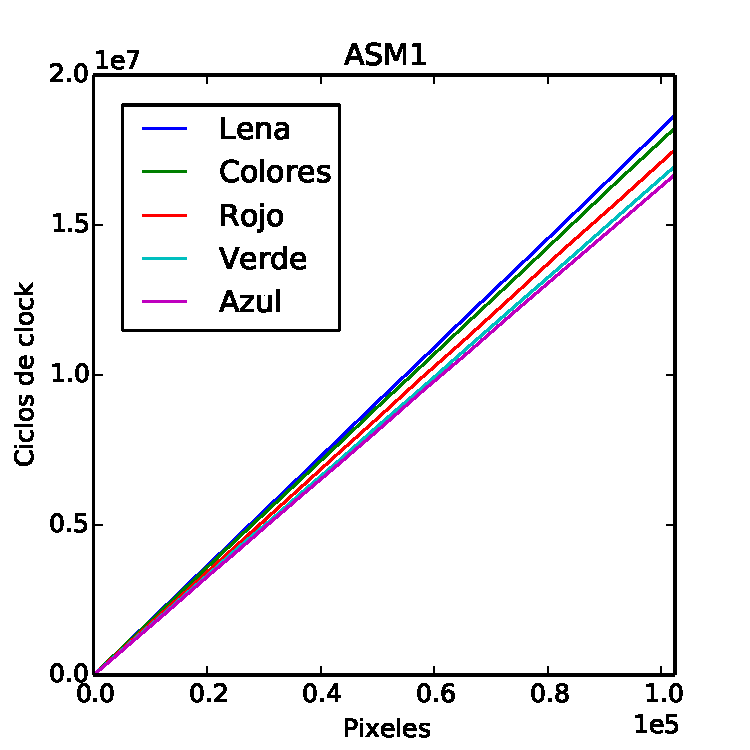
\includegraphics[scale=0.45]{images/asm1_hsl_lena_colors}
% 	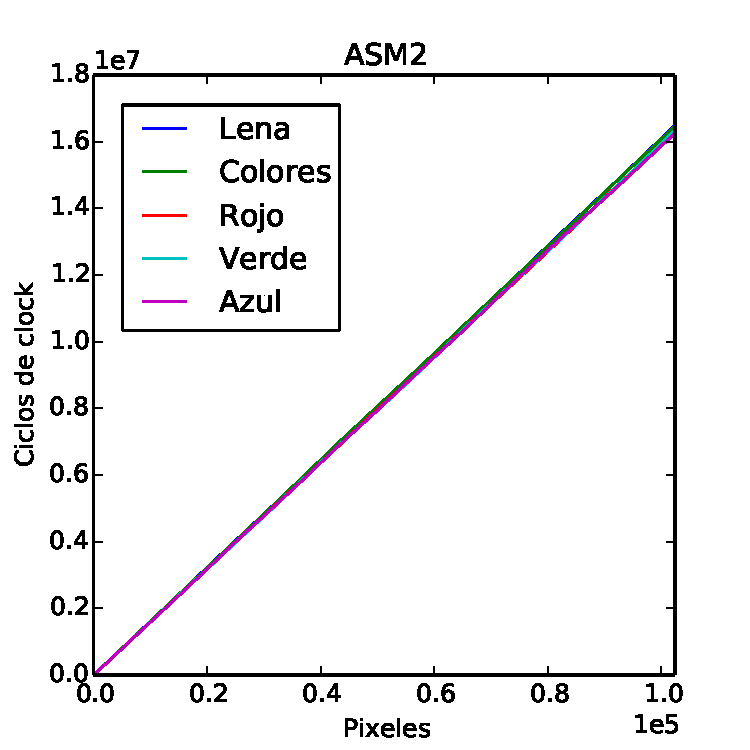
\includegraphics[scale=0.45]{images/asm2_hsl_lena_colors}
% \end{figure}

% Como podemos ver, la segundo implementacion (que no usa ningun tipo de condicional) se matuvo constante independientemente del contenido de la imagen, mientras que la de $C$ y la primer implementacion en $Assembler$, que emplean condicionales tuvieron una diferencia considerable en resultados. De todas formas, la implementacion de $C$ termino siendo la de mejor rendimiento.

% Para el segundo test se obtvieron los siguientes resultados:\\

% \begin{figure}[h!]
% 	\centering
% 	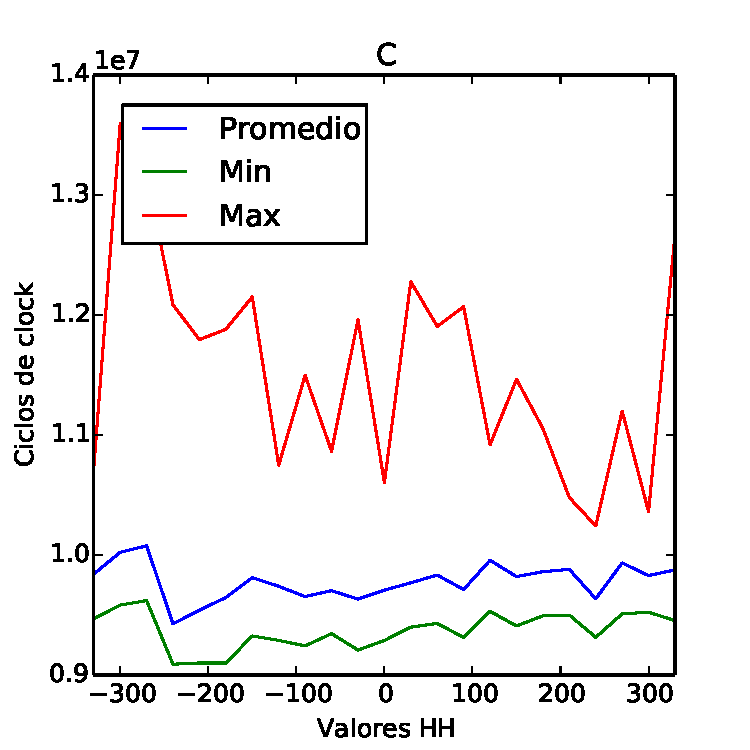
\includegraphics[scale=0.45]{images/c_lenahsl}
% 	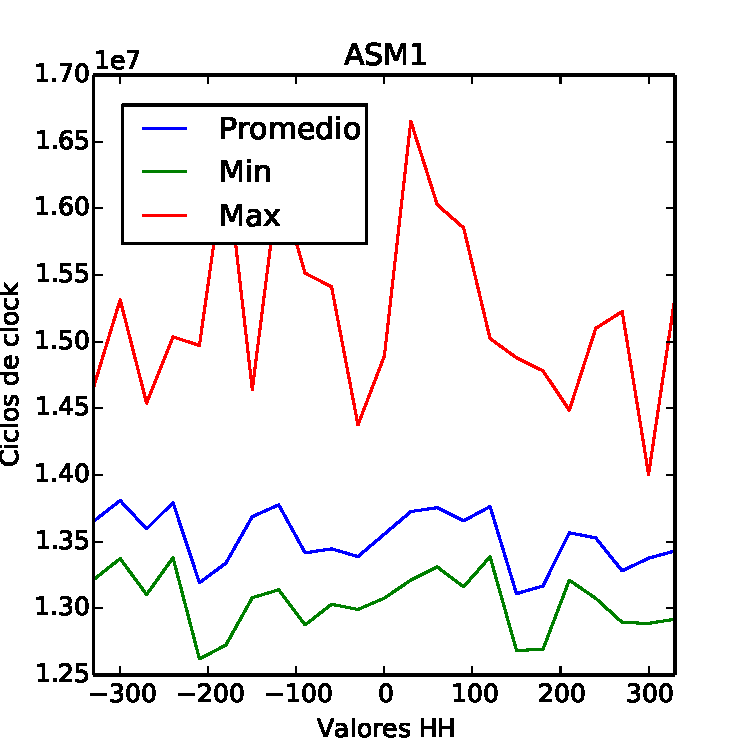
\includegraphics[scale=0.45]{images/asm1_lenahsl}
% 	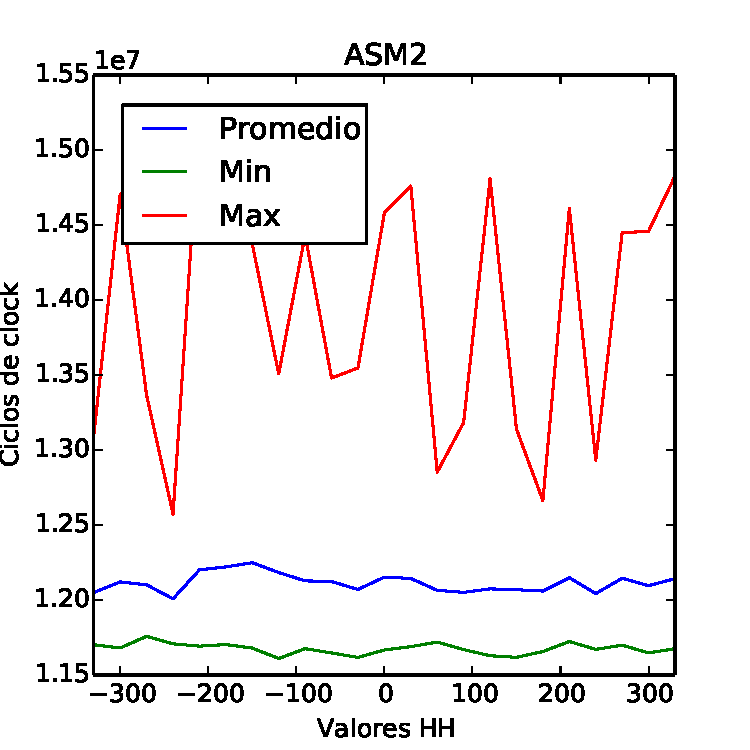
\includegraphics[scale=0.45]{images/asm2_lenahsl}
% \end{figure}

% Aqui podemos ver que el valor de \texttt{HH} no afecta en gran manera al rendimiento, ya que la cantidad de ciclos se mantiene relativamente constante independientemente del \texttt{HH}, y al igual que el primer test, la implementacion de $C$ sigue teniendo mejor rendimiento.

\subsection{Conclusion}
Aqui nos encontramos con un caso donde el paralelismo de SIMD no nos ayudo a mejorar el rendimiento, sino que lo empeoro. La cantidad de condicionales sobre cada una de las componentes del pixel hace que la aritmetica de las implementaciones de SSE tome una cantidad muy grande de ciclos de clock.

A pesar de su rendimiento, nos parece importante destacar que la implementacion $ASM2$ se ejecuto en un tiempo muy similar para las diferentes imagenes, en casos donde la consistencia sea mas valorada que la eficiencia se podria hacer uso de esta implementacion.

%En conclusion podemos ver que la version de C es la mas rapida, suponemos que esto es asi debido a que la prediccion de saltos del procesador es lo suficientemente buena como para que sea mas rapido que hacer las cosas usando SIMD y procesando todo usando mascaras.

%Tambien podemos ver tambien que los saltos afectan la consistencia del algoritmo ya que la implementacion ASM2 posee tiempos de ejecucion mucho mas consistentes, en cambio la de C y ASM1 (La cual posee funciones con saltos) poseen variaciones en los tiempos de ejecucion.

% Este filtro trajo varias sorpresas respecto al rendimiento, si bien los condicionales afectaron en mayor o menor medida a la implementacion en $C$, esta termino siendo la mejor en practicamente todos los casos probados. Consideramos que esto se debe a que el trabajo que realiza el filtro no era amigable al paralelismo, es decir, muchas veces se realizaban calculos que luego terminan siendo filtrado por alguna mascara.
\newpage

\end{document}